\documentclass[12pt]{article}
\usepackage{pifont}
\usepackage{a4wide}
\usepackage[utf8x]{inputenc}
\usepackage{amsmath}
\usepackage{amsfonts}
\usepackage{mathrsfs}
%\usepackage{natbib}
\usepackage{graphicx} % figuras
%\usepackage[export]{adjustbox} % loads also graphicx
\usepackage{float}
\usepackage[font=footnotesize]{caption}
\usepackage{wrapfig}
\usepackage{authblk}
\usepackage{subfigure}

\usepackage{amssymb}
\usepackage{latexsym}
\usepackage[sort&compress]{natbib}



\topmargin=-2pt
\title{On POD-based Deflation Vectors for DPCG applied to porous media problems.}

\author[1]{G. B. Diaz Cortes}  
\author[1]{C. Vuik} 
\author[2]{J. D. Jansen} 
\affil[1]{Department of Applied Mathematics, TU Delft}
\affil[2]{Department of Geoscience \& Engineering, TU Delft}
\renewcommand\Authands{ and }
\date{April 2017}


\begin{document}
% \thispagestyle{empty}
% \noindent
% \begin{center}
% {\Large \sc DELFT UNIVERSITY OF TECHNOLOGY}
% \\
% \vspace{3cm}
% {\large \sc REPORT 17-01}\\[4ex]
% {\large \sc On POD-based Deflation Vectors for DPCG applied to porous media problems.}\\[4ex]
% {\large \sc G. B. Diaz Cortes, C. Vuik, J. D. Jansen}\\
% \vfill
% {\tt ISSN 1389-6520}\\[2ex]
% {\tt Reports of the Delft Institute of Applied Mathematics}\\[2ex]
% {\tt Delft 2017}
% \end{center}
% \pagebreak
% \thispagestyle{empty}
% \vspace*{\fill}
% \noindent
% \hspace*{-0,3cm}Copyright~~~\Pisymbol{psy}{227}~~~2017 by Delft Institute of Applied Mathematics, Delft, \mbox{The Netherlands.}
% \\[2ex]
% No part of the Journal may be reproduced, stored in a retrieval system, or
% transmitted, in any form or by any means, electronic, mechanical, photocopying,
% recording, or otherwise, without the prior written permission from Delft Institute of
% Applied Mathematics, Delft University of Technology, The
% Netherlands. 
% % newpage, title etc.
% \setcounter{page}{1}
\newpage
\maketitle
\begin{abstract}
     We study fast and robust iterative solvers for large systems of linear equations resulting from simulation of flow trough strongly heterogeneous porous media. We propose the use of preconditioning and deflation techniques, based on information obtained from the system, to reduce the time spent in the solution of the linear system.\\
     An important question when using deflation techniques is how to find good deflation vectors, which lead to a decrease in the number of iterations and a small increase in the required computing time per iteration. In this paper, we propose the use of deflation vectors based on a POD-reduced set of snapshots. We investigate convergence and the properties of the resulting methods. 
     Finally, we illustrate these theoretical results with numerical experiments.  
 We consider compressible and incompressible single-phase flow in a layered model with variations in the permeability layers up to $10^{3}$ and the SPE 10 benchmark model with a contrast in permeability coefficients of $10^{7}$. Using deflation for the incompressible problem, we reduce the number of iterations to 1 or 2 iterations. With deflation, for the compressible problem, we reduce up to $\sim 80\%$ the number of iterations when compared with the only-preconditioned solver.\\
\end{abstract}
\newpage
 \section{Introduction.}
  Often, most computational time in the simulation of multi-phase flow through porous media is taken 
  up by the solution of the pressure equation. 
This involves, primarily, solving large systems of linear equations as part of the iterative solution of the time and space discretized governing nonlinear partial differential 
equations. The time spent in solving the linear systems depends on the size of the problem and the heterogeneity, i.e. the spatial
variations of rock permeability values within the medium (permeability is an inverse measure of the resistance to flow which is related to the porosity and the pore structure of the rock). Solution of problems with extreme contrasts in the
permeability values may lead to very large computing times. \\
Iterative methods are known to be the best option to solve such extreme problems. However, sometimes iterative methods are not sufficient to solve these problems in a reasonable amount of time. As the systems become larger or ill-conditioned, finding a way to accelerate the convergence of these methods becomes necessary. Preconditioning is a way to accelerate convergence, but new preconditioning techniques still need to be developed to improve the performance of iterative methods \cite{Vuik02,Benzi02}.
Reduced Order Models (ROM) have also been studied to improve computational efficiency by reducing the model size without losing essential information \cite{Antoulas05,Schilders08,Quarteroni14}. 
A potential ROM to reduce the computing time for large-scale problems is Proper Orthogonal 
Decomposition (POD), a method that has been investigated for flow problems in porous media in \cite{Heijn04,Vermeulen04,Mark06,Doren06,Cardoso09,Astrid11,Krogstad11,Efendiev12,Jiang13,Pasetto16} among others. 
The use of a POD-based preconditioner for acceleration of the solution is proposed by Astrid et al.
\cite{Astrid11} to solve the pressure equation resulting from two-phase reservoir simulation, by Jiang et al. \cite{Jiang13} for a similar application and by Pasetto 
et al. \cite{Pasetto16} for groundwater flow models. \\
The POD method requires the computation of a series of 'snapshots' which are solutions of the problem with slightly 
different parameters or well inputs. Astrid et al. \cite{Astrid11} use snapshots in the form of solutions of the pressure equation computed in a small number of short pre-simulations, prior to the actual simulation,\ with diverse well configurations, reporting promising speed ups with factors between three and five. They note that the overhead required to pre-compute the POD solutions implies that the method will be particularly attractive when many solutions of near-similar simulation models are required. A similar approach is followed by Jiang \cite{Jiang13}, who concludes that POD-based pressure preconditioning does not appear to be an ideal choice because of its dependence on the differences between the right-hand sides (forcing terms) used in the pre-simulations and the actual simulation. The snapshots computed by Pasetto et al. \cite{Pasetto16} are solutions of the previous time steps in the full-model.
Once the snapshots are computed, the POD method is used to obtain a set of basis vectors that capture the most relevant features of the system, which can be used to speed-up the subsequent simulations.\\
The method of Pasetto at al. \cite{Pasetto16} is partly based on the work of Markovinovic and Jansen \cite{Mark06} who use a similar, but more restricted, approach in which the acceleration is 
achieved by only improving the initial guess.\\
Problems with high contrast between the permeability coefficients are sometimes approached through the use of deflation techniques, see, e.g., \cite{Vuik99}. These techniques involve the search of good deflation vectors, which are usually problem-dependent. In \cite{Vuik99}, subdomain based deflation vectors are used for layered problems with a large contrast between permeability coefficients. However, 
these deflation vectors cannot be used if the distribution of the permeability coefficients is not structured, as is usually the case in reservoir simulation models; see, e.g., the well-known SPE 10 benchmark problem \cite{Christie01}.\\
Algebraic Multigrid (AMG)\cite{Klie07}, Multi-level and Domain Decomposition \cite{Tang09} preconditioners have been studied in combination deflation techniques to accelerate the convergence of iterative methods.
In \cite{Mark06,Astrid11} and \cite{Pasetto16}, after computing a basis from the previously obtained snapshots, the solution is computed in the subspace generated by this basis and then projected back to the original high-dimensional system. Carlberg et al. \cite{Carlberg15} also use POD to obtain information from the system, in particular, the previous time step solutions. Then, a Krylov-subspace is constructed using the information obtained previously.\\
Following the ideas of \cite{Astrid11,Mark06,Pasetto16,Carlberg15}, we propose the use of POD of many snapshots to capture the system's behavior and combine this technique with deflation to accelerate the convergence of an iterative Krylov method.
In this work, instead of computing the solution in a low dimensional subspace, the basis obtained with POD is proposed as an alternative choice for the deflation vectors to accelerate the convergence of the pressure solution in reservoir simulation.  \\
This work is divided into six sections. 
  Section \ref{fpm} is devoted to a detailed description of the models used to simulate flow through a porous medium. In Section \ref{syseq}, we present some theory about the linear solvers used in this work and we introduce preconditioning 
  and deflation techniques. 
  In Section \ref{POD} we present some theory about POD. We prove two lemmas that will help us in the choice of good deflation vectors for the 
  incompressible case in Section \ref{as}.\\
 In Section \ref{numexp} we present numerical experiments. We describe the problem that is studied, the solver and the preconditioning and deflation techniques used to speed up the solver. The results are also presented in this section.
 Finally, we end with the conclusions.
 \newpage
 \section{Flow through porous media}\label{fpm}
When simulating flow of two phases through a porous medium, these two phases can be considered as separated, i.e., they are inmiscible and there is no mass transfer between them. 
The contact area between phases is known as the interface.\\ 
While modeling two phases, we 
usually consider one of the fluids as the wetting phase ($w$) which is more attracted to the mineral particles than the other phase.
The other phase is consider as non-wetting phase ($n$). In the case of a water-oil system, water is considered
the wetting phase. \\
% For a reservoir, the density of each phase varies, the gas is less dense than the oil and water. 
% Therefore, the gas is found on top of the reservoir. For the oil-water system, water's density is larger 
% than oil's, then water is found on the bottom of the reservoir.\\
The saturation of a phase $S_{\alpha},$ is the fraction of void space filled with that phase in a porous 
medium. If the phase is not present, we have a cero saturation of that phase.
If there are two phases present in the porous medium, these fluids fill completely the empty space, which is
expressed by the following relation.
\begin{equation}\label{eq:satrel}
 S_n+S_w=1
\end{equation}
The surface tension and the curvature of the interface between the fluids causes a difference in pressure
between the two phases. 
% The pressure in the wetting fluid is less than in the nonwetting fluid. 
This difference in pressures is known as the capillary pressure, $p_c$, which, depends on the saturation:
\begin{equation}\label{eq:cappress}
 p_c(S_w)=p_n-p_w.
\end{equation}
The pressure in the non-wetting fluid is higher than the pressure in the wetting fluid, 
therefore, the capillary pressure is always a positive quantity. 
The relation between the capillary pressure and the saturation is obtained as an empirical model based on experiments. 
The capillary curve depends on the difference in pore-size 
distributions, porosity and permeability of the medium.
To normalize the measured data, it's common to use a function called Leverett J-function, which takes the following 
form:

\begin{equation}
 J(S_w)=\frac{P_c}{\sigma cos \theta}\sqrt{\frac{K}{\phi}},
\end{equation}
where $\sigma$ is the surface tension and $\theta$ the contact angle.\\
Sometimes, the capillary pressure is expressed as an analytical function of the normalized water saturation ($ \hat{S}_w =\frac {S_w-S_w^ {min}}{S_w^ {max}-S_w^{min}}$).
A model for the relationship between the capillary pressure and water saturation was proposed by Brooks and Corey:
\begin{equation*}
\hat{S}_w=
\begin{cases}
(p_c/p_e)^{-n_b} & \text{ if } p_c>p_e\\
1& p_c \leq p_e
\end{cases}
\end{equation*}
where $p_e$ is the entry pressure of air, and $n_b$ is related to the pore-size distribution.
Another model was proposed by Genuchten:
\begin{equation}
 \hat{S}_w=\left( 1+(\beta_gp_c)^n_g)^{-m_g}\right),
\end{equation}
where $\beta_g$ is related to the average size of pores and $n_g$ and $m_g$ are related to the pore size distribution. \\
\emph{Relative permeability}\\
When modelling two phases, the permeability of each phase, $\alpha$ will be affected by the presence of the other phase, therefore an effective permeability $K_\alpha$ for each phase has to be used instead of the absolute permeability $K$.  
Due to interfacial tensions, the sum of all the phase permeabilities is less than one.
$$\sum_{\alpha}K_{\alpha}^e<K.$$
The saturation dependent relative permeability is defined as:
$$k_{r\alpha}(S)=K_{\alpha}^e/K.$$
The simplest model possible that relates the relative permeabilities with the saturations is the is Corey model:
\begin{equation}\label{eq:Corey}
\begin{aligned}
k_{rw}=(\hat{S}_w)^{n_w}k_w^0,\\
k_{ro}=(1-\hat{S}_w)^{n_n}k_o^0.\\
\end{aligned}
\end{equation}
where $n_w>1$, $n_o>1$ and $k_{\alpha}^0$ are fitting parameters.\\
% The Brooks-Corey functions are also used. 
% \begin{equation*}
% \begin{aligned}
% k_{rw}=(\hat{S}_w)^{n_1+n_2n_3},\\
% k_{ro}=(1-\hat{S}_w)^{n_1}[1-(\hat{S}_w)^{n_2}]^{n_3}.\\
% \end{aligned}
% \end{equation*}
% where, $n_1 = 2$, $n_2 = 1 + 2/n_b$ and $n4 = 1$ for the Brooks–Corey–Burdine model and $n_1 = \eta$, $n_2 = 1 + 1/n_b$ and $n3 = 2$ for the Brooks–Corey–Mualem model. For the van Genuchten capillary functions $m_g = 1 − 1/n_g$) we have:
% \begin{equation*}
% \begin{aligned}
% k_{rw}=\hat{S}_w^2[1-(1-\hat{S}_w^{1/m_g})^{m_g}],\\
% k_{ro}=(1-\hat{S}_w)^2[1-(\hat{S}_w^{1/m_g})]^{m_g},\\
% \end{aligned}
% \end{equation*}
% which is called the Genuchten-Burdine model.\\
% If we have an oil reservoir  with volume $V$ and porosity $\phi$ the oil volume
% in reservoir (OIP-oil in place) is given by:
% $$OIP=V\phi (1-S_{wc})$$
% Where $S_{wc}$ is the irreducible water saturation, the water present in the oil and gas zones of the
% reservoir, also known as connate water. 
% If the oil is generated in deep rock, when it moves to an upper 
% zone filled with water, it cannot displace all the water. This water remain as connate water, normally 
% between 10 and 15 \%.
As in the single-phase case, the governing equations for two-phase flow in a porous medium are the mass conservation and Darcy's law. 
The mass balance equations for each phase $\alpha$ are given by:
\begin{equation}\label{eq:mb2ph}
 \frac{\partial(\phi \rho_{\alpha}S_{\alpha})}{\partial t}+\nabla \cdot ( \rho_{\alpha} \mathbf{v}_{\alpha})=\rho_{\alpha} q_{\alpha},
\end{equation}
Darcy's law is:
\begin{equation}\label{eq:D2ph}
\mathbf{v}_{\alpha}=-\frac{k_{r\alpha}}{\mu_{\alpha}} {K}(\nabla p_{\alpha}-\rho_{\alpha} g \nabla z).
\end{equation}
To simplify notation, the phase mobilities ($\lambda_{\alpha}=Kk_{r\alpha}/\mu_{\alpha}$) or relative phase mobilities ($\lambda_{\alpha}=\lambda_{\alpha}K$) are used. 
Combining Darcy's law \eqref{eq:D2ph} and mass balance \eqref{eq:mb2ph} equations and using the phase mobilities, the system reads:
\begin{equation}\label{eq:2ph}
 \frac{\partial(\phi \rho_{\alpha}S_{\alpha})}{\partial t}-\nabla \cdot ( \rho_{\alpha} \lambda_{\alpha}(\nabla p_{\alpha}-\rho_{\alpha} g \nabla z))=\rho_{\alpha} q_{\alpha}.
\end{equation}




% Using the discrete derivative operators and backward discretization of temporal derivatives, the resulting system of discrete equations is:
% \begin{equation*}
%  \frac{(\phi \mathbf{\rho}_{\alpha}\mathbf{S}_{\alpha})^{n+1}-(\phi \mathbf{\rho}_{\alpha}\mathbf{S}_{\alpha})^{n}}{\Delta t^n}+\nabla \cdot  ( \mathbf{\rho}_{\alpha} \mathbf{v}_{\alpha})^{n+1}= \mathbf{q}_{\alpha}^{n+1},
% \end{equation*}
% 
% \begin{equation*}
% \mathbf{v}_{\alpha}^{n+1}=-\frac{\mathbf{k}_{r\alpha}}{\mathbf{\mu}_{\alpha}} \mathbf{K}[\nabla( \mathbf{p}_{\alpha}^{n+1})-g\mathbf{\rho}_{\alpha}^{n+1}  \nabla(\mathbf{z})].
% \end{equation*}

\emph{Incompressible two-phase flow}\\

In the case of incompressible flow, the porosity $\phi$ and the densities $\rho_{\alpha}$ doesn't depend on time. Therefore, Equation \eqref{eq:2ph} reduces to: 
\begin{equation}\label{eq:2ph}
 \phi \frac{\partial S_{\alpha}}{\partial t}-\nabla \cdot (  \lambda_{\alpha}(\nabla p_{\alpha}-g \nabla z))= q_{\alpha}.
\end{equation}
A common approach to solve this problem is the fractional flow formulation, where the fractional flow function is defined as $$f_{\alpha1}=\frac{\lambda_{\alpha1}}{\lambda_{\alpha1}+\lambda_{\alpha2}}.$$
\emph{Fractional flow formulation}\\
Part of the non linearity of previous formulation can be eliminated if the system is expressed in terms of one phase pressure and one phase saturation. A common choice is to use $p_n$ and $S_w$ which gives the following system
\begin{equation}
 \frac{\partial(\phi \rho_{w}{S}_{w})}{\partial t}+\nabla \cdot ( \rho_{w} \frac{{K}k_{rw}}{\mu_w}(\nabla p_n-\nabla P_c(S_w)-\rho_w g \nabla z))=\rho_{w} q_{w},
\end{equation}
\begin{equation}
 \frac{\partial(\phi \rho_{n}(1-{S}_{w}))}{\partial t}+\nabla \cdot ( \rho_{n} \frac{{K}k_{rn}}{\mu_n}(\nabla p_n-\rho_n g \nabla z))=\rho_{n} q_{n}.
\end{equation}

\emph{Incompressible flow}\\
For incompressible flow, only the Saturation $S$ is a function of time and the fluid densities $\rho_{\alpha}$ are constant. Therefore, the mass-balance equations are:
\begin{equation}
 \phi\frac{\partial( {S}_{\alpha})}{\partial t}+\nabla \cdot ( \mathbf{v}_{\alpha})= q_{\alpha}.
\end{equation}
The total Darcy velocity is defined as the sum of the velocity in the wetting and non wetting phases, it can be expressed in terms of the non-wetting phase as:
\begin{align*}
\mathbf{v}=\mathbf{v}_w+\mathbf{v}_n=-\lambda_{n}\nabla p_n-\lambda_{w}\nabla p_w+(\lambda_n \rho_n+\lambda_w\rho_w)g\nabla z\\
=-(\lambda_n+\lambda_w)\nabla p_n+\lambda_w\nabla p_c+(\lambda_n \rho_n+\lambda_w\rho_w)g\nabla z
\end{align*}
if we add the two continuity equations and use the relationship $S_n+S_w=1$ we have:
\begin{equation*}
 \phi\frac{\partial( {S}_{w}+S_n)}{\partial t}+\nabla \cdot ( \mathbf{v}_{w}+\mathbf{v}_n)= q_{n}+q_w.
\end{equation*}
Using $\lambda=\lambda_n+\lambda_w=\lambda K$ as the total mobility and $q=q_n+q_w$ as the total source, for the total Darcy velocity we have:
\begin{align*}
-\nabla \cdot (\lambda K\nabla p_n)=q-\nabla[\lambda_w\nabla p_c+(\lambda_n\rho_n+\lambda_w\rho_w)g\nabla z].
\end{align*}
Multiplying each phase velocity by the relative mobility of the other phase and subtracting the result we obtain:
\begin{align*}
\lambda_n\mathbf{v}_w-\lambda_w\mathbf{v}_n&=\lambda\mathbf{v}_w-\lambda_w\mathbf{v}\\
&=\lambda_w\lambda_n K[\nabla p_c+(\rho_w-\rho_n)g\nabla z].
\end{align*}
Therefore, for $\mathbf{v}_w$ we have
\begin{align*}
\mathbf{v}_w=\frac{\lambda_w}{\lambda}\mathbf{v}+\frac{\lambda_w\lambda_n}{\lambda} K[\nabla p_c+(\rho_w-\rho_n)g\nabla z].
\end{align*}
Using the velocity computed above, for the wetting phase we have:
\begin{equation}\label{eq:sat}
 \phi\frac{\partial( {S}_{w})}{\partial t}+\nabla \cdot [f_w( \mathbf{v}+\lambda_n\Delta  \rho g\nabla z)]= q_w-\nabla \cdot(f_w\lambda_np_c\nabla S_w).
\end{equation}
with $\Delta \rho= \rho_w-\rho_n$ and the fractional flow function $f_w$:
$$f_w=\frac{\lambda_{w}}{\lambda_n+\lambda_w},$$
is the fraction of the total flow that consists of the wetting fluid, and
\begin{align*}
\mathbf{v}=-\lambda(\nabla p_n-f_w\nabla p_w-(f_n \rho_n+f_w\rho_w)g\nabla z)\\
\end{align*}

The coupling between the elliptic pressure equation and the parabolic saturation equation is much weaker than the coupling between the two continuity
equations in the two-pressure formulation. In the pressure equation,
the coupling to saturation appears explicitly in the effective mobility that makes up the variable coefficient in the Poisson problem and on the
right-hand side through the phase mobilities and the derivative of the capillary function. In Equation \eqref{eq:sat}, the saturation is only indirectly
coupled to the pressure through the total Darcy velocity. \\
The system of PDEs can then be reformulated so that
it consists of an elliptic equation for fluid pressure and one or more transport equations. These transport equations are generally parabolic, but have a
strong hyperbolic character. Since the pressure and saturations equations have very different mathematical characteristics, it is natural
to solve them in consecutive substeps. Sequential solution procedures and in-
compressible flow models are popular in academia and for research purposes,
but are less used in industry. To the extent simulations are used for practical reservoir engineering, they are mainly based on compressible equations
and solution procedures in which flow and transport are solved as a coupled
system. Such approaches are very robust and particularly useful for problems
with large variations in time constants or strong coupling between different
types of flow mechanisms. \\\\\\


\emph{Immiscible two-phase flow}\\
For the case of immiscible fluids, the flow equations are:
\begin{equation}\label{we}
 \frac{\partial(\phi \rho_{w}S_{w})}{\partial t}+\nabla \cdot ( \rho_{w} \mathbf{v}_{w})=\rho_{w} q_{w},
\end{equation}
\begin{equation}\label{ne}
 \frac{\partial(\phi \rho_{n}S_{.})}{\partial t}+\nabla \cdot ( \rho_{n} \mathbf{v}_{n})=\rho_{n} q_{n}.
\end{equation}
\emph{Pressure formulation}\\
We can choose the pressures as the primary unknowns, then the saturations are expressed as functions of pressure. 
Assuming the capillary pressure has a unique inverse function $\hat{S}_w=P_c^{-1}(p_c)$, then we have:
$$S_w=\hat{S}_w(p_n-p_w)\qquad S_n=1-\hat{S}_w(p_n-p_w), $$
then equations \eqref{we} and \eqref{ne} can be written as:
\begin{equation}
 \frac{\partial(\phi \rho_{w}\hat{S}_{w})}{\partial t}+\nabla \cdot ( \rho_{w} \frac{{K}k_{rw}(\hat{S}_w)}{\mu_w}(\nabla p_w-\rho_w g \nabla z))=\rho_{w} q_{w},
\end{equation}
\begin{equation}
 \frac{\partial(\phi \rho_{n}(1-\hat{S}_{w}))}{\partial t}+\nabla \cdot ( \rho_{n} \frac{{K}k_{rn}(\hat{S}_w)}{\mu_n}(\nabla p_n-\rho_n g \nabla z))=\rho_{n} q_{n}.
\end{equation}
Previous system is highly coupled and strongly nonlinear. \\
\emph{Fractional flow formulation}\\
Part of the non linearity of previous formulation can be eliminated if the system is expressed in terms of one phase pressure and one phase saturation. A common choice is to use $p_n$ and $S_w$ which gives the following system
\begin{equation}
 \frac{\partial(\phi \rho_{w}{S}_{w})}{\partial t}+\nabla \cdot ( \rho_{w} \frac{{K}k_{rw}}{\mu_w}(\nabla p_n-\nabla P_c(S_w)-\rho_w g \nabla z))=\rho_{w} q_{w},
\end{equation}
\begin{equation}
 \frac{\partial(\phi \rho_{n}(1-{S}_{w}))}{\partial t}+\nabla \cdot ( \rho_{n} \frac{{K}k_{rn}}{\mu_n}(\nabla p_n-\rho_n g \nabla z))=\rho_{n} q_{n}.
\end{equation}

\emph{Incompressible flow}\\
For incompressible flow, only the Saturation $S$ is a function of time and the fluid densities $\rho_{\alpha}$ are constant. Therefore, the mass-balance equations are:
\begin{equation}
 \phi\frac{\partial( {S}_{\alpha})}{\partial t}+\nabla \cdot ( \mathbf{v}_{\alpha})= q_{\alpha}.
\end{equation}
The total Darcy velocity is defined as the sum of the velocity in the wetting and non wetting phases, it can be expressed in terms of the non-wetting phase as:
\begin{align*}
\mathbf{v}=\mathbf{v}_w+\mathbf{v}_n=-\lambda_{n}\nabla p_n-\lambda_{w}\nabla p_w+(\lambda_n \rho_n+\lambda_w\rho_w)g\nabla z\\
=-(\lambda_n+\lambda_w)\nabla p_n+\lambda_w\nabla p_c+(\lambda_n \rho_n+\lambda_w\rho_w)g\nabla z
\end{align*}
if we add the two continuity equations and use the relationship $S_n+S_w=1$ we have:
\begin{equation*}
 \phi\frac{\partial( {S}_{w}+S_n)}{\partial t}+\nabla \cdot ( \mathbf{v}_{w}+\mathbf{v}_n)= q_{n}+q_w.
\end{equation*}
Using $\lambda=\lambda_n+\lambda_w=\lambda K$ as the total mobility and $q=q_n+q_w$ as the total source, for the total Darcy velocity we have:
\begin{align*}
-\nabla \cdot (\lambda K\nabla p_n)=q-\nabla[\lambda_w\nabla p_c+(\lambda_n\rho_n+\lambda_w\rho_w)g\nabla z].
\end{align*}
Multiplying each phase velocity by the relative mobility of the other phase and subtracting the result we obtain:
\begin{align*}
\lambda_n\mathbf{v}_w-\lambda_w\mathbf{v}_n&=\lambda\mathbf{v}_w-\lambda_w\mathbf{v}\\
&=\lambda_w\lambda_n K[\nabla p_c+(\rho_w-\rho_n)g\nabla z].
\end{align*}
Therefore, for $\mathbf{v}_w$ we have
\begin{align*}
\mathbf{v}_w=\frac{\lambda_w}{\lambda}\mathbf{v}+\frac{\lambda_w\lambda_n}{\lambda} K[\nabla p_c+(\rho_w-\rho_n)g\nabla z].
\end{align*}
Using the velocity computed above, for the wetting phase we have:
\begin{equation}\label{eq:sat}
 \phi\frac{\partial( {S}_{w})}{\partial t}+\nabla \cdot [f_w( \mathbf{v}+\lambda_n\Delta  \rho g\nabla z)]= q_w-\nabla \cdot(f_w\lambda_np_c\nabla S_w).
\end{equation}
with $\Delta \rho= \rho_w-\rho_n$ and the fractional flow function $f_w$:
$$f_w=\frac{\lambda_{w}}{\lambda_n+\lambda_w},$$
is the fraction of the total flow that consists of the wetting fluid, and
\begin{align*}
\mathbf{v}=-\lambda(\nabla p_n-f_w\nabla p_w-(f_n \rho_n+f_w\rho_w)g\nabla z)\\
\end{align*}

The coupling between the elliptic pressure equation and the parabolic saturation equation is much weaker than the coupling between the two continuity
equations in the two-pressure formulation. In the pressure equation,
the coupling to saturation appears explicitly in the effective mobility that makes up the variable coefficient in the Poisson problem and on the
right-hand side through the phase mobilities and the derivative of the capillary function. In Equation \eqref{eq:sat}, the saturation is only indirectly
coupled to the pressure through the total Darcy velocity. \\
The system of PDEs can then be reformulated so that
it consists of an elliptic equation for fluid pressure and one or more transport equations. These transport equations are generally parabolic, but have a
strong hyperbolic character. Since the pressure and saturations equations have very different mathematical characteristics, it is natural
to solve them in consecutive substeps. Sequential solution procedures and in-
compressible flow models are popular in academia and for research purposes,
but are less used in industry. To the extent simulations are used for practical reservoir engineering, they are mainly based on compressible equations
and solution procedures in which flow and transport are solved as a coupled
system. Such approaches are very robust and particularly useful for problems
with large variations in time constants or strong coupling between different
types of flow mechanisms. \\\\\\
\emph{\textbf{Sequential solution procedures}}\\
The two-phase, incompressible model will be solved using the fractional-flow formulation. This fractional flow model consists of an elliptic
pressure equation
\begin{equation}\label{eq:wdarcy}
 \nabla \cdot \mathbf{v}=q, \qquad \mathbf{v}=-\lambda(\nabla p_n-f_w\nabla p_c-(f_n \rho_n+f_w\rho_w)g\nabla z)\\
\end{equation}
and a parabolic transport equation \eqref{eq:sat}
\begin{equation}\label{eq:wsat}
 \phi\frac{\partial( {S}_{w})}{\partial t}+\nabla \cdot [f_w( \mathbf{v}+\lambda_n(\Delta  \rho g\nabla z)+\nabla P_c)]= q_w.
\end{equation}
Where the capillary pressure $p_c = p_w −p_n$ is assumed to be a known function $P_c$ of the wetting saturation $S_w$. The transport equation becomes hyperbolic whenever $P_c$ is zero.\\
In the standard sequential solution procedure, the system above, is
evolved in time using a set of discrete time steps $\Delta t_i$ . We assume that $p, \mathbf{v},$
and $S_w$ are all known at time t and that we want to evolve the solution to time
$t + \Delta t$.\\
At the beginning of the time step, we first assume that the saturation
$S_w$ is fixed. This means that the parameters $\lambda, f_w ,$ and $f_n$ are 
functions of the spatial variable $\mathbf{x}$, and hence we can use this equation only to update the pressure $p_n$ and the Darcy velocity $\mathbf{v}$. Then, $\mathbf{v}$ and $p_n$ are held
fixed while equation \ref{eq:wsat} is evolved a time step $\Delta t$ to define an updated saturation $S_w (\mathbf{x}, t + \Delta t)$. This saturation is then held fixed when we update $p_n$ and $\mathbf{v}$ in the next time step, and so on.
Some authors refer to this solution procedure as an operator splitting
method since the solution procedure effectively splits the overall solution operator of the flow model into two parts that are evolved in consecutive substeps.
Likewise, some authors refer to the sequential solution procedure as IMPES,
which is short-hand for implicit pressure, explicit saturation. Using the name
IMPES is strictly speaking only correct if the saturation evolution is approximated by a single time step of an explicit transport solver.\\\\
\emph{\textbf{Pressure solvers}}\\
The pressure Equation \eqref{eq:wdarcy} for incompressible, multiphase flow is time dependent. This time dependence comes as the result of three factors:
\begin{enumerate}
 \item $K/\mu$ being replaced by the total mobility $\lambda(S_w )$, which depends on time through the saturation $S_w (\mathbf{x}, t + \Delta t)$,
 \item the constant density $\rho$ being replaced by a saturation-dependent quantity $\rho_w f_w (S_w ) + \rho_nf_n (S_w )$, and
 \item the source term $q$ being replaced by a saturation-dependent source term
$q − \nabla \lambda_w (S_w )\nabla P_c (S_w )$.
\end{enumerate}
However, once $S_w$ is held fixed in time, all three quantities become functions of $\mathbf{x}$ only, and we hence end up again with an elliptic Poisson-type equation having the same spatial variation. \\
\emph{Saturation solvers}\\
The saturation equation depends on the time, using backward Euler discretization for the time derivative in Equation \ref{eq:wsat}, we have:
\begin{equation}\label{eq:wsat1}
 \phi\frac{( {S}_{w}^{n+1}-{S}_{w}^n)}{\Delta t}+\nabla \cdot [f_w({S}_{w})( \mathbf{v}+\lambda_n({S}_{w})(\Delta  \rho g\nabla z+\nabla P_c({S}_{w})))]= q_w,
\end{equation}
or
\begin{equation*}\label{eq:wsat2}
 {S}_{w}^{n+1}={S}_{w}^n-\frac{\Delta t}{\phi}\nabla \cdot [f_w({S}_{w})( \mathbf{v}+\lambda_n({S}_{w})(\Delta  \rho g\nabla z+\nabla P_c({S}_{w})))]+q_w,
\end{equation*}
which can be computed explicitly:
\begin{equation*}\label{eq:wsat3}
 {S}_{w}^{n+1}={S}_{w}^n-\mathcal{F}({S}_{w}^{n},{S}_{w}^{n}),
\end{equation*}
or implicitly:
\begin{equation*}\label{eq:wsat4}
 {S}_{w}^{n+1}={S}_{w}^n-\mathcal{F}({S}_{w}^{n+1},{S}_{w}^{n}).
\end{equation*}
If we use the implicit scheme, the system is nonlinear and depends on the saturation at time step $n$ and $n+1$.\\
The discretization is implemented with the following residual form for each cell $\Omega_i$,
\begin{equation}\label{eq:resS}
 F_i (s, r) = s_i − r_i +\frac{\Delta t}{\phi_i|\Omega_i|}[H_i (s) − max(q_i, 0) − min(q_i , 0)f (S_i )],
\end{equation}
where $s$ and $r$ are cell-averaged quantities and subscript $i$ refers to
the cell the average is evaluated in. The sum of the interface fluxes for cell $i$ 
\begin{equation}
 H_i (s) =\sum_k \frac{\lambda^u_w (s_i , s_k )}{\lambda^u_w (si , sk ) + \lambda^u_n (si , sk )}[v_{ik} + \lambda^u_n (s_i , s_k )(g_{ik} + P_{ik} )],
\end{equation}
is computed using the single-point upstream mobility-weighting, whereas the fractional flow function $f$ in the source term
is evaluated from the cell average of $S$ in cell $\Omega_i$ . The explicit scheme is given
as $S^{n+1} = S^n −F(S^n , S^n )$ and the implicit solution is obtained solving $F(S^{n+1} , S^{ n}) = 0$. 
The residual equations \eqref{eq:resS} for all cells in vector form
\begin{equation}
 \mathbf{F} (\mathbf{s}) = \mathbf{s} − \mathbf{S} +\frac{\Delta t}{\phi_i|\Omega|}[\mathbf{H} (\mathbf{s}) − \mathbf{Q}^+ − \mathbf{Q}^-\mathbf{f} (\mathbf{S} )]=\mathbf{0}.
\end{equation}
Here, s is the unknown state at time $tf$ and S is the known state at the start
of the time step. The nonlinear system can be solved with NR method, where, for the $(k+1)$-th iteration we have:

$$\mathbf{J}(\mathbf{S}^k)\delta\mathbf{S}^{k+1}=-\mathbf{F}(\mathbf{S}^k;\mathbf{S}^n),
\qquad \mathbf{S}^{k+1}=\mathbf{S}^k+\delta \mathbf{S}^{k+1},$$
where $\mathbf{J}(\mathbf{S}^k)=\frac{\partial \mathbf{F}(\mathbf{S}^k;\mathbf{S}^n)}{\partial \mathbf{S}^k}$ is the 
Jacobian matrix, and $\delta \mathbf{S}^{k+1}$ is the NR update at iteration step $k+1$.\\
Therefore, the linear system to solve is:\\
\begin{equation}\label{eq:lsS}
\mathbf{J}(\mathbf{pS}^k)\delta \mathbf{S}^{k+1}=\mathbf{b}(\mathbf{S}^k).
\end{equation}
with $\mathbf{b}(\mathbf{S}^k)$ being the function evaluated at iteration step $k$, $\mathbf{b}(\mathbf{S}^k)=-\mathbf{F}(\mathbf{S}^k;\mathbf{S}^n)$.\\

% \newpage
% \newpage
% \section{Iterative solution methods}\label{syseq}
% When simulating single-phase flow through a porous medium, we obtain a linear system
% \begin{equation}\label{eq:linsys}
%  \mathbf{A}\mathbf{x}=\mathbf{b},
% \end{equation}
% for both compressible and incompressible models. 
% Since $\mathbf{A}$ is SPD, we choose Conjugate Gradient (CG) as iterative method accelerated with the Incomplete Cholesky preconditioner. In this work, we also study the acceleration with deflation techniques. In this section, we give a brief overview of the methods. \\\\
% \textbf{Conjugate Gradient Method}\\
% Given a starting solution $\mathbf{x}^0$ and the residual defined by $\mathbf{r}^k=\mathbf{b}-\mathbf{A}\mathbf{x}^k$, we define the Krylov subspace 
% $\mathcal{K}_k(\mathbf{A},\mathbf{r}^0)=span\{\mathbf{r}^0,\mathbf{A}\mathbf{r}^0,\dots,\mathbf{A}^{k-1}\mathbf{r}^0\}$ and $\mathbf{x}^k\in \mathbf{x}^0+\mathcal{K}_k(\mathbf{A},\mathbf{r}^0)$ has a minimal error measured in the $\mathbf{A}$-norm for all approximations contained in $\mathbf{x}^0+\mathcal{K}_k(\mathbf{A},\mathbf{r}^0).$ The error of this approximation is bounded by:
% \begin{equation}\label{eq:conv1}
%  ||\mathbf{x}-\mathbf{x}^{k+1}||_\mathbf{A}\leq 2||\mathbf{x}-\mathbf{x}^{0}||_\mathbf{A} 
%  \left( \frac{\sqrt{\kappa_2(\mathbf{A})}-1}{\sqrt{\kappa_2(\mathbf{A})}+1} \right)^{k+1}
%  \footnote{The condition number $\kappa_2(\mathbf{A})$ is defined as  $\kappa_2(\mathbf{A})=
%  \frac{\sqrt{\lambda_{max}(\mathbf{A}^T\mathbf{A})}}{\sqrt{\lambda_{min}(\mathbf{A}^T\mathbf{A})}}$. 
%  If $\mathbf{A}$ is SPD, $\kappa_2(\mathbf{A})=\frac{\lambda_{max}(\mathbf{A})}{\lambda_{min}(\mathbf{A})}$.}.
%  \end{equation}
%  The pseudo code for CG is given in Algorithm 2.\\
%  \begin{table}[!h]
% \begin{tabular}{ |l| } 
% \hline
%   \textbf{Algorithm 2} Conjugate Gradient (CG) method, solving $\mathbf{A}\mathbf{x}=\mathbf{b}$.\\
%   \hline
%  \hline
% \\
% Give an initial guess $\mathbf{x}^0$. \\Compute $\mathbf{r}^0=\mathbf{b}-\mathbf{A}\mathbf{x}^0$ and set $\mathbf{p}^0=\mathbf{r}^0$.\\
% 
% \hspace{0.5cm}\textbf{for} $k=0,...,$ until convergence\\
%  \hspace{1cm} $\alpha^k=\frac{(\mathbf{r}^{k},\mathbf{r}^{k})}{(\mathbf{A}\mathbf{p}^k,\mathbf{p}^k)}$\\
% \hspace{1cm} $\mathbf{x}^{k+1}=\mathbf{x}^k+\alpha^k\mathbf{p}^k$\\
% \hspace{1cm}$\mathbf{r}^{k+1}=\mathbf{r}^k-\alpha^k\mathbf{A}\mathbf{p}^k$\\
% \hspace{1cm}$ \beta^k=\frac{(\mathbf{r}^{k+1},\mathbf{r}^{k+1})}{(\mathbf{r}^k,\mathbf{r}^k)}$\\
% \hspace{1cm}$\mathbf{p}^{k+1}=\mathbf{r}^{k+1}+\beta^k\mathbf{p}^k$\\
% \hspace{0.5cm}\textbf{end}\\
% \hline
% \end{tabular}
% \end{table}
% \newpage
% \textbf{Preconditioning}\\
% \hspace{0.5cm}To accelerate the convergence of a Krylov method, one can transform the system into
% another one containing an iteration matrix with a better spectrum , i.e, a smaller condition number. 
% This can be done by multiplying the system \eqref{eq:linsys} by a matrix $\mathbf{M}^{-1}.$
% \begin{equation}\label{eq:precon}
%  \mathbf{M}^{-1}\mathbf{A}\mathbf{x}=\mathbf{M}^{-1}\mathbf{b}.
% \end{equation}
% The new system has the same solution but can provide a substantial reduction of the condition number. 
% For this preconditioned system, the error is bounded by:
% \begin{equation}\label{eq:convp}
%  ||\mathbf{x}-\mathbf{x}^{k}||_\mathbf{A}\leq 2||\mathbf{x}-\mathbf{x}^{0}||_\mathbf{A} 
%  \left( \frac{\sqrt{\mathbf{\kappa}(\mathbf{M}^{-1}\mathbf{A})}-1}{\sqrt{\mathbf{\kappa}(\mathbf{M}^{-1}\mathbf{A})}+1} \right)^{k}.
% \end{equation}
% $\mathbf{M}$ is chosen as an $SPD$ matrix such that $\mathbf{\kappa}(\mathbf{M}^{-1}\mathbf{A})\leq \mathbf{\kappa}(\mathbf{A}),$ and $\mathbf{M}^{-1}\mathbf{b}$ is cheap to compute.\\\\
% \textbf{Deflation}\\
% Deflation is used to annihilate the effect of extreme eigenvalues on the convergence of an iterative method (\cite{Vuik99}). 
% Given an $SPD$ matrix $\mathbf{A} \in \mathbb{R}^{n \times n}$, for a given matrix $\mathbf{Z}\in \mathbb{R}^{n\times m}$ the deflation matrix $\mathbf{P}$ is defined as follows (\cite{Tang08,Tang09}):
% $$\mathbf{P}=\mathbf{I}-\mathbf{A}\mathbf{Q}, \qquad \mathbf{P} \in \mathbb{R}^{n \times n}, \qquad \mathbf{Q} \in \mathbb{R}^{n \times n},$$
% where
% $$\mathbf{Q}=\mathbf{Z}\mathbf{E}^{-1}\mathbf{Z}^T, \qquad \mathbf{Z} \in \mathbb{R}^{n \times m}, \qquad \mathbf{E} \in \mathbb{R}^{m \times m}, $$
% with
% $$\mathbf{E}=\mathbf{Z}^T\mathbf{A}\mathbf{Z}.$$
% The matrix $\mathbf{E}$ is known as the $Galerkin$ or $coarse$ matrix that has to be invertible. 
% If $\mathbf{A}$ is $SPD$ and $\mathbf{Z}$ is full rank then $\mathbf{E}$ is invertible. 
% The full rank matrix $\mathbf{Z}$ is called the $deflation-subspace$ matrix, 
% and it's columns are the
% $deflation$ vectors or $projection$ vectors.\\
% \textbf{Deflated PCG Method}\\
% \hspace{0.5cm}To obtain the solution of linear system \eqref{eq:linsys}, we have to solve the deflated system (see Appendix \ref{a4}):
% \begin{align}\label{eq:defsol}
% \mathbf{P}\mathbf{A} \hat{\mathbf{x}}=\mathbf{P}\mathbf{b},
% \end{align}
% with the CG method, for the deflated solution $\hat{\mathbf{x}}$. 
% This deflated the solution is related to the solution $\mathbf{x}$ of the original system as (see Appendix \ref{a4}):
% \begin{equation}\label{eq:xfromxh}
%     \mathbf{x}=\mathbf{Q}\mathbf{b}+\mathbf{P}^T\mathbf{\hat{x}}.
% \end{equation}
% The deflated linear system can also be preconditioned by an $SPD$ matrix $\mathbf{M}$. After preconditioning, the deflated preconditioned system to solve with CG is \cite{Tang09}:
% $$\tilde{\mathbf{P}} \tilde{\mathbf{A}} \hat{\tilde{\mathbf{x}}}=\tilde{\mathbf{P}}\tilde{\mathbf{b}},$$
% where:
% \begin{equation*}
%  \tilde{\mathbf{A}}=\mathbf{M}^{-\frac{1}{2}}\mathbf{A}\mathbf{M}^{-\frac{1}{2}}, \qquad \hat{\tilde{\mathbf{x}}}=\mathbf{M}^{\frac{1}{2}}\hat{\mathbf{x}}, \qquad
%  \tilde{\mathbf{b}}=\mathbf{M}^{-\frac{1}{2}}\mathbf{b}
% \end{equation*}
% This method is called the Deflated Preconditioned Conjugate Gradient $DPCG$ method.
% In practice $\mathbf{M}^{-1}\mathbf{P}\mathbf{A}\mathbf{x}=\mathbf{M}^{-1}\mathbf{P}\mathbf{b}$ is computed and the error is bounded by:
% \begin{equation*}
%  ||\mathbf{x}-\mathbf{x}^{i+1}||_\mathbf{A}\leq 2||\mathbf{x}-\mathbf{x}^{0}||_\mathbf{A} \left( \frac{\sqrt{\mathbf{\kappa}_{eff}(\mathbf{M}^{-1}\mathbf{P}\mathbf{A})}-1}{\sqrt{\mathbf{\kappa}_{eff}(\mathbf{M}^{-1}\mathbf{P}\mathbf{A})}+1} \right)^{i+1},
% \end{equation*}
% were $\mathbf{\kappa}_{eff}=\frac{\lambda_{max}(M^{-1}PA)}{\lambda_{min}(M^{-1}PA)}$ is the effective condition 
% number and $\lambda_{min}(M^{-1}PA)$ is the smallest non-zero eigenvalue of $M^{-1}PA$.
% 
% \subsection{Choices of Deflation Vectors}
% \hspace{0.5cm}The deflation method is used to remove the effect of the most unfavorable eigenvalues
% of $\mathbf{A}$. If the matrix $\mathbf{Z}$ contains eigenvectors corresponding to the unfavorable 
% eigenvalues, the convergence of the 
% iterative method is achieved faster. However, to obtain and to apply the eigenvectors is costly in view of memory and CPU time.
% Therefore, a good choice of the matrix $\mathbf{Z}$ that efficiently approximate the eigenvectors is essential
% for the applicability of the method.\\
% A good choice of the deflation vectors is usually problem-dependent. Available information on the system is, in general,
% used to obtain these vectors.
% Most of the techniques used to choose deflation vectors are based on approximating eigenvectors, 
% recycling \cite{Clemens04}, subdomain deflation vectors \cite{Vuik02} or multigrid and 
% multilevel based deflation techniques \cite{Tang09,Smith96}. A summary of these techniques is given below.
% \begin{description}
%  \item [Recycling Deflation.] A set of search vectors previously used is reused to build the deflation-subspace 
%  matrix \cite{Clemens04}. 
% The vectors could be, for example, $q-1$
% solution vectors of the linear system with different right-hand sides or of different time steps.
% The matrix $\mathbf{Z}$ containing these solutions is:
% $$\mathbf{Z}=[\mathbf{x}^{(1)},\mathbf{x}^{(2)},...,\mathbf{x}^{(q-1)}].$$
%  \item [Subdomain Deflation.] The domain is divided into several subdomains,
%  using domain decomposition techniques or taking into account the properties of the problem.
% For each subdomain, there is a deflation vector that contains ones for cells in the 
% subdomain and zeros for cells outside \cite{Vuik02}.
%  \item [Multi Grid and Multilevel Deflation.] For the multigrid and multilevel methods, 
%  the prolongation and restriction matrices are used to pass from one level or grid to another. 
% These matrices can be used as the deflation-subspace matrices $\mathbf{Z}$ \cite{Tang09}.
% \end{description}
% \newpage
% \section{Proper Orthogonal Decomposition (POD)}\label{POD}
% 
% \hspace{0.5cm}
% As mentioned before, in this work we want to combine deflation techniques and Proper Orthogonal Decomposition method (POD) to reduce the number of iterations necessary to solve the linear system obtained from reservoir simulation in a cheap and automatic way. In this section, we give a brief overview of the POD method.\\
% The POD method is a Model Order Reduction (MOR) method, where a high-order model is projected onto a space
% spanned by a small set of orthonormal basis vectors.
% The high dimensional variable $\mathbf{x} \in \mathbb{R}^n$
% is approximated by a linear combination of $l$ orthonormal basis vectors \cite{Astrid11}:
% \begin{equation}\label{eq4}
%   \mathbf{x}\approx \sum_{i=1}^lc_i \mathbf{\psi}_i,
% \end{equation}
% where $\psi_i \in \mathbb{R}^n$ are the basis vectors and $c_i$ are their corresponding coefficients.
% In matrix notation, equation \eqref{eq4} is rewritten as :
% $$\mathbf{x}\approx \Psi\mathbf{c},$$
% where $\Psi=[\psi_1 \text{ }\psi_2 \text{ }.. \text{ }\psi_l]$, $\Psi \in \mathbb{R}^{n\times l}$ 
% is the matrix containing the basis vectors, and $\mathbf{c} \in \mathbb{R}^l$ is the vector 
% containing the coefficients of the basis vectors. \\
% The basis vectors $\psi_i$ are computed from a set of 'snapshots' $\{ \mathbf{x_i}\} _{i=1,..,m}$, 
% obtained by simulation or experiments \cite{Mark06}. 
% In POD, the basis vectors $\{ \mathbf{\psi} _j \} ^l _{j=1},$ are $l$ eigenvectors corresponding to 
% the largest eigenvalues $\{ \mathbf{\sigma} _j \} ^l _{j=1}$ of the data snapshot correlation matrix $\mathbf{R}$.
% \begin{equation}\label{eq:POD}
% \mathbf{R}:= \frac{1}{m}\mathbf{X}\mathbf{X}^T \equiv \frac{1}{m} \sum_{i=1}^m \mathbf{x}_i \mathbf{x}_i^T,
% \qquad \mathbf{X}:=[\mathbf{x}_1,\mathbf{x}_2,...\mathbf{x}_m],
% \end{equation}
% where $\mathbf{X}\in \mathbb{R}^{n\times m}$ is an SPSD matrix containing the previously obtained snapshots.
% The $l$ eigenvectors should contain almost all the variability of the snapshots. 
% Usually, they are chosen as the eigenvectors of the maximal number ($l$) of eigenvalues satisfying \cite{Mark06}:
% \begin{equation}
% \frac{\sum_{j=1}^l\sigma_j}{\sum_{j=1}^m\sigma_j}\leq \alpha, \qquad 0<\alpha \leq 1,
% \end{equation}
% with $\alpha$ close to 1. The eigenvalues $\sigma_j$ are ordered from large to small with $\sigma_1$
% the largest eigenvalue of $\mathbf{R}$. 
% It is not necessary to compute the eigenvalues from $\mathbf{X}\mathbf{X}^T$, instead, it is possible to compute the eigenvalues of the much smaller matrix $\mathbf{X}^T\mathbf{X}$ (see Appendix \ref{a3}). \\
% % The covariance matrix $\bar{\mathbf{R}}$ (see Equation \eqref{eq:POD1}) is frequently used instead of $\mathbf{R}$.
% % \begin{equation}\label{eq:POD1}
% % \bar{\mathbf{R}}:=  \frac{1}{m} \sum_{i=1}^m (\mathbf{x}_i -\bar{\mathbf{x}})(\mathbf{x}_i-\bar{\mathbf{x}})^T,
% % \qquad \bar{\mathbf{x}}:=\frac{1}{m} \sum_{i=1}^m\mathbf{x}_i.
% % \end{equation}
% In this study, we normalize the snapshots, so $||\mathbf{x}_i||_2=1.$

\newpage
\section{Numerical experiments}\label{numexp}
\subsection{Model problems}\label{modpro}
\hspace{0.5cm} We model water floding into a reservoir initially filled with oil. Therefore, the initial saturation is set as 1 for the oil and 0 for the water (see Figure \ref{fig:initsat1}, and Table \ref{table:sat}). 
The solution of the systems of linear equations resulting from the discretization of partial differential equations for the description of this process is studied in this work. 
The solution of the system is performed with the Deflated Conjugate Gradient method preconditioned with Incomplete Cholesky (DICCG).
We propose the use of snapshots and the snapshots-based POD vectors as deflation vectors for the above-mentioned method.\\The matrices corresponding to the linear systems $\mathbf{A}$ and right-hand sides $\mathbf{b}$ are obtained with the Matlab Reservoir Simulation Toolbox (MRST) \cite{Lie13}.
\\
In the present section, we give a general overview of the experiments that we perform, but the specifications are presented below for each problem separately. 
\subsection*{Heterogeneous permeability layers}
The experiments simulate flow through a porous medium with a constant porosity field of 0.2.
For the first set of experiments, we study a layered system (see Figure \ref{fig:rockperm1}). We use 8 layers of the same size, 
4 layers with one value of permeability $\sigma_1$, followed by a layer with a different permeability value $\sigma_2$. The permeability of one set of layers is set to $\sigma_1=1mD$, the permeability of the other set $\sigma_2$ is varied. 
Therefore, the contrast in permeability between the layers $(\frac{\sigma_2}{\sigma_1}=\sigma_2)$,
depends on the value of $\sigma_2$.
The permeability $\sigma_2$ varies from $\sigma_2=10^{-1}mD$ to $\sigma_2=10^{-3}mD$. 
The domain consists of a Cartesian grid of 64 x 64 cells with a length of one meter each cell. For the relative permeability of the fluids, the Corey model is used. The properties of the fluids are presented in Table \ref{table:fluids}. No gravity terms and no capillary pressure are taken into account in the first set of experiments.
For the second set, capillary pressure is taken into account. And finally, we perform 3D experiments with 64 x 64 x 10 grid cells and gravity terms are included. 
\begin{table}[!ht]
\hspace{1cm}
\begin{minipage}{.9\textwidth}%\hspace{-1cm}
\centering
\begin{tabular}{ |c|c|c|c|} 
\hline
Property&Water&Oil&Units\\
\hline
$\mu$&     1&    10 & $cp$  \\  
$\rho$& 1000& 700& $kg/m^3$\\
$k_r$&$(S_w)^2$&   $(1-S_w)^2$ &  \\
\hline
\end{tabular}
\caption{Fluids properties.}\label{table:fluids}
\end{minipage} \hspace{1cm} 
\end{table} 


\begin{figure}[!h] \hspace{-1cm}
\begin{minipage}{.3\textwidth}
 \centering
\includegraphics[width=4cm,height=4cm,keepaspectratio]
{/mnt/sda2/cortes/Results/17_04/two_phases/19/bcx/10-7_64nz1perm_1cp0/def_0_pod_0/Permeability.jpg}
\caption{Rock permeability}
\label{fig:rockperm1}
\end{minipage}%  
\hspace{0.5cm}
\begin{minipage}{.3\textwidth}
 \centering
\includegraphics[width=4cm,height=4cm,keepaspectratio]
{/mnt/sda2/cortes/Results/17_04/two_phases/19/bcx/10-7_64nz1perm_1cp0/def_0_pod_0/RelPerm.jpg}
\caption{Fluid relative permeability}
\label{fig:Convho}
\end{minipage}%
\hspace{0.7cm}
\begin{minipage}{.4\textwidth}
\centering
\includegraphics[width=5cm,height=5cm,keepaspectratio]
{/mnt/sda2/cortes/Results/17_04/two_phases/19/bcx/10-7_64nz1perm_1cp0/def_0_pod_0/ISat.jpg}
\vspace{-0cm}
\caption{ Initial saturation}
\label{fig:initsat1}
\end{minipage}
\end{figure}

\emph{\textbf{Injection through the boundary}}\\
For the first set of experiments, water is injected from one boundary at a rate of $0.1$ $m^3/day$ and pressure is set as zero at the right boundary and 100 bars inside the reservoir. In Case 1 the water is injected from the left boundary, and in Case 2, water is injected from the bottom boundary. The simulation is run during 4800 days with a time step of 40 days (See Table \ref{table:ic}).  

\begin{table}[!ht]
\begin{minipage}{.4\textwidth}
\centering
\begin{tabular}{ |c|c|c|} 
\hline
\multicolumn{3}{|c|}{Case 1}\\
\hline
&Water&Oil\\
\hline
$S_{0,x\neq 0, L_x}$&0&1\\
$S_{x=0}$&1&0\\
$S_{x=L_x}$&0&1\\
\hline
\multicolumn{3}{|c|}{Case 2}\\
\hline
&Water&Oil\\
\hline
$S_{0,y\neq 0, L_y}$&0&1\\
$S_{y=0}$&1&0\\
$S_{y=L_y}$&0&1\\
\hline
\end{tabular}
\caption{Saturations.}\label{table:sat}
\end{minipage}%
\hspace{1cm}
\begin{minipage}{.4\textwidth}
%\begin{table}[!ht]
\centering
\begin{tabular}{ |c|c|c|} 
\hline
Property&Value&Units\\
\hline
    $T_{total}$&     4800& days\\
$dT$& T/120&days\\
\hline
\multicolumn{3}{|c|}{Case 1}\\
\hline
$Q_{x=0}$&0.1&$m^3/day$\\
$P_{0,x\neq 0, L_x}$&100&$bars$\\
$P_{x=L_x}$&0&$bars$\\
\hline
\multicolumn{3}{|c|}{Case 2}\\
 \hline
 $Q_{y=0}$&0.1&$m^3/day$\\
$P_{0,y\neq 0, L_y}$&100&$bars$\\
$P_{y=L_y}$&0&$bars$\\
\hline
\end{tabular}\caption{Initial values of the system.}
\label{table:ic}
\end{minipage}
\end{table} 

\emph{The solver}\\
The solution of the system is approximated with the ICCG and DICCG methods. \\
For the DICCG method, it is necessary to select a set of deflation vectors. In the first series of experiments, the deflation vectors are the solutions of the system in the previous 10 time steps (DICCG$_{10}$). The snapshots of the first 10 time steps are obtained with ICCG.
For the second set of experiments POD is used (DICCG$_{POD_{10}}$). In the first case 10 (DICCG$_{POD_{10}}$), and in the second 5 POD vectors (DICCG$_{POD_{5}}$) are used as deflation vectors.
As tolerance or stopping criterium we use the relative residual, defined as the 2-norm of the residual of the $k^{th}$ iteration divided by 
the 2-norm of the right-hand side of the preconditioned system: 
$$\frac{||\mathbf{M}^{-1}r^k||_2}{||\mathbf{M}^{-1}b||_2}\leq \epsilon.$$
The stopping criterium of the linear solvers is $10^{-7}$. 

\subsubsection*{Case 1: Injection through the left boundary, no capillary pressure.}
In Table \ref{table:liter1}, the number of iterations necessary to achieve convergence are presented for various contrast between permeability layers for the deflation method with different selection of deflation vectors. The number of iterations necessary to achieve convergence for the ICCG method is presented in the second column (Total ICCG). The number of iterations necessary to compute the first 10 snapshots with the ICCG method are presented in the 4th column (ICCG Snapshots). In the 5th column, we present the total number of iterations taking into account the first 10 snapshots computed with ICCG and the rest of the iterations computed with DICCG. In the last column, the percentage of the total number of iterations of the DICCG methods with respect to the ICCG method is presented.   
The pressure field and the saturations for oil and water are presented in Figures \ref{fig:p1} and \ref{fig:sat1} for various times.
\begin{table}[!h]\centering
\begin{minipage}{1\textwidth}
 \centering
\begin{tabular}{ ||c|c||l|c|c|c|c||} 
\hline
$\frac{\sigma_2}{\sigma_1}$&Total&Method  & ICCG&DICCG &Total&\% of total\\ 
                           & ICCG     &  & Snapshots& &ICCG& ICCG\\ 
                            &     &  & & &+DICCG& \\
\hline 
$10^{1}$ &13109& DICCG$_{10}$&950&1653&2603&20\\ 
\hline  
$10^{1}$ &13109& DICCG$_{POD_{10}}$&950&1655&2605&20 \\ 
\hline  
$10^{1}$ &13109& DICCG$_{POD_{5}}$&950&1770&2720&21 \\ 
\hline  
$10^{2}$ &13429& DICCG$_{10}$&902&1475&2377&18\\ 
\hline  
$10^{2}$ &13429& DICCG$_{POD_{10}}$&902&1475&2377&18 \\ 
\hline  
$10^{2}$ &13429& DICCG$_{POD_{5}}$&902&1499&2401&18 \\ 
\hline 
$10^{3}$ &10612& DICCG$_{10}$&602&1142&1744&16\\ 
\hline  
$10^{3}$ &10612& DICCG$_{POD_{10}}$&602&1142&1744&16 \\ 
\hline  
$10^{3}$ &10612& DICCG$_{POD_{5}}$&602&1130&1732&16 \\ 
\hline  
\end{tabular} 
\caption{Comparison between the ICCC and DICCG methods of the average number of linear iterations for various contrast between permeability layers. Injection through the left boundary, domain 64 x 64 cells.}\label{table:liter1} 
\end{minipage}  
\end{table}  

\begin{figure}[!h]
\begin{minipage}{.9\textwidth}
\vspace{0cm}
\centering
%\hspace{2cm}
\includegraphics[width=15cm,height=15cm,keepaspectratio]
{/mnt/sda2/cortes/Results/17_04/two_phases/19/bcx/10-7_64nz1perm_1cp0/def_0_pod_0/Pressure.jpg}
\vspace{-0cm}
\caption{Pressure field for various times for a contrast between permeability values of $10^{1}$, 64 x 64 grid cells.}
\label{fig:p1}
\end{minipage}
\end{figure}
\begin{figure}[!h]
\begin{minipage}{.9\textwidth}
\vspace{0cm}
\centering
%\hspace{2cm}
\includegraphics[width=15cm,height=15cm,keepaspectratio]
{/mnt/sda2/cortes/Results/17_04/two_phases/19/bcx/10-7_64nz1perm_1cp0/def_0_pod_0/Sat.jpg}
\vspace{-0cm}
\caption{Saturations of oil and water for various times for a contrast between permeability values of $10^{1}$, 64 x 64 grid cells.}
\label{fig:sat1}
\end{minipage}
\end{figure}
\begin{figure}[!h]
\begin{minipage}{.9\textwidth}
\vspace{0cm}
\centering
%\hspace{2cm}
\includegraphics[width=7cm,height=7cm,keepaspectratio]
{/mnt/sda2/cortes/Results/17_04/two_phases/19/bcx/10-7_64nz1perm_1cp0/def_0_pod_0/Estcondnumb.jpg}
\vspace{-0cm}
\caption{Estimated condition number of the matrix A for a contrast between permeability values of $10^{1}$, 64 x 64 grid cells.}
\label{fig:cn1}
\end{minipage}
\end{figure}


\newpage
\subsubsection*{Case 1 A: Injection through the left boundary, capillary pressure included.}
In Table \ref{table:liter1a} the number of iterations necessary to achieve convergence are presented for various contrast between permeability layers for the deflation method with different selection of deflation vectors. The number of iterations necessary to achieve convergence for the ICCG method is presented in the second column (Total ICCG). The number of iterations necessary to compute the first 10 snapshots with the ICCG method are presented in the 4th column (ICCG Snapshots). In the 5th column, we present the total number of iterations taking into account the first 10 snapshots computed with ICCG and the rest of the iterations computed with DICCG. In the last column, the percentage of the total number of iterations of the DICCG methods with respect to the ICCG method is presented.   
The pressure field and the saturations for oil and water are presented in Figures \ref{fig:p1a} and \ref{fig:sat1a} for various times.
\begin{table}[!h]\centering
\begin{minipage}{1\textwidth}
 \centering
\begin{tabular}{ ||c|c||l|c|c|c|c||} 
\hline
$\frac{\sigma_2}{\sigma_1}$&Total&Method  & ICCG&DICCG &Total&\% of total\\ 
                           & ICCG     &  & Snapshots& &ICCG& ICCG\\ 
                            &     &  & & &+DICCG& \\
\hline 
$10^{1}$ &12712& DICCG$_{10}$&949&1065&2014&16\\ 
\hline  
$10^{1}$ &12712& DICCG$_{POD_{10}}$&949&1065&2014&16 \\ 
\hline  
$10^{1}$ &12712& DICCG$_{POD_{5}}$&949&1125&2074&16 \\ 
\hline  
$10^{2}$ &12450& DICCG$_{10}$&894&1049&1943&16\\ 
\hline  
$10^{2}$ &12450& DICCG$_{POD_{10}}$&894&1049&1943&16 \\ 
\hline  
$10^{2}$ &12450& DICCG$_{POD_{5}}$&894&1059&1953&16 \\ 
\hline  
$10^{3}$ &9790& DICCG$_{10}$&600&893&1493&15\\ 
\hline  
$10^{3}$ &9790& DICCG$_{POD_{10}}$&600&893&1493&15 \\ 
\hline  
$10^{3}$ &9790& DICCG$_{POD_{5}}$&600&839&1439&15 \\ 
\hline
\end{tabular} 
\caption{Comparison between the ICCC and DICCG methods of the average number of linear iterations for various contrast between permeability layers. Injection through the left boundary, domain 64 x 64 cells, capillary pressure included.}\label{table:liter1a} 
\end{minipage}  
\end{table}  

\begin{figure}[!h]
\begin{minipage}{.9\textwidth}
\vspace{0cm}
\centering
%\hspace{2cm}
\includegraphics[width=15cm,height=15cm,keepaspectratio]
{/mnt/sda2/cortes/Results/17_04/two_phases/19/bcx/10-7_64nz1perm_1cp1/def_0_pod_0/Pressure.jpg}
\vspace{-0cm}
\caption{Pressure field for various times for a contrast between permeability values of $10^{1}$, 64 x 64 grid cells, capillary pressure included.}
\label{fig:p1a}
\end{minipage}
\end{figure}
\begin{figure}[!h]
\begin{minipage}{.9\textwidth}
\vspace{0cm}
\centering
%\hspace{2cm}
\includegraphics[width=15cm,height=15cm,keepaspectratio]
{/mnt/sda2/cortes/Results/17_04/two_phases/19/bcx/10-7_64nz1perm_1cp1/def_0_pod_0/Sat.jpg}
\vspace{-0cm}
\caption{Saturations of oil and water for various times for a contrast between permeability values of $10^{1}$, 64 x 64 grid cells, capillary pressure included.}
\label{fig:sat1a}
\end{minipage}
\end{figure}
\begin{figure}[!h]
\begin{minipage}{.9\textwidth}
\vspace{0cm}
\centering
%\hspace{2cm}
\includegraphics[width=7cm,height=7cm,keepaspectratio]
{/mnt/sda2/cortes/Results/17_04/two_phases/19/bcx/10-7_64nz1perm_1cp1/def_0_pod_0/Estcondnumb.jpg}
\vspace{-0cm}
\caption{Estimated condition number of the matrix A for a contrast between permeability values of $10^{1}$, 64 x 64 grid cells.}
\label{fig:cn1a}
\end{minipage}
\end{figure}
\subsubsection*{Case 1 B: Injection through the left boundary, no capillary pressure, gravity included (3D).}
In Table \ref{table:liter1b} the number of iterations necessary to achieve convergence are presented for various contrast between permeability layers for the deflation method with different selection of deflation vectors. The number of iterations necessary to achieve convergence for the ICCG method is presented in the second column (Total ICCG). The number of iterations necessary to compute the first 10 snapshots with the ICCG method are presented in the 4th column (ICCG Snapshots). In the 5th column, we present the total number of iterations taking into account the first 10 snapshots computed with ICCG and the rest of the iterations computed with DICCG. In the last column, the percentage of the total number of iterations of the DICCG methods with respect to the ICCG method is presented.   
The pressure field and the saturations for oil and water are presented in Figures \ref{fig:p1b} and \ref{fig:sat1b} for various times.
\begin{table}[!h]\centering
\begin{minipage}{1\textwidth}
 \centering
\begin{tabular}{ ||c|c||l|c|c|c|c||} 
\hline
$\frac{\sigma_2}{\sigma_1}$&Total&Method  & ICCG&DICCG &Total&\% of total\\ 
                           & ICCG     &  & Snapshots& &ICCG& ICCG\\ 
                            &     &  & & &+DICCG& \\
\hline 
$10^{1}$ &30662& DICCG$_{10}$&1210&616&1826&6\\ 
\hline  
$10^{1}$ &30662& DICCG$_{POD_{10}}$&1210&482&1692&6 \\ 
\hline  
$10^{1}$ &30662& DICCG$_{POD_{5}}$&1210&590&1800&6 \\ 
\hline  
$10^{2}$ &33843& DICCG$_{10}$&1195&669&1864&6\\ 
\hline  
$10^{2}$ &33843& DICCG$_{POD_{10}}$&1195&682&1877&6 \\ 
\hline  
$10^{2}$ &33843& DICCG$_{POD_{5}}$&1195&795&1990&6 \\ 
\hline 
$10^{3}$ &27144& DICCG$_{10}$&695&856&1551&6\\ 
\hline  
$10^{3}$ &27144& DICCG$_{POD_{10}}$&695&897&1592&6 \\ 
\hline  
$10^{3}$ &27144& DICCG$_{POD_{5}}$&695&1008&1703&6 \\ 
\hline
\end{tabular} 
\caption{Comparison between the ICCC and DICCG methods of the average number of linear iterations for various contrast between permeability layers. Injection through the left boundary, domain 64 x 64 x 10 cells, no capillary pressure, gravity  included.}\label{table:liter1b} 
\end{minipage}  
\end{table}  

\begin{figure}[!h]
\begin{minipage}{.9\textwidth}
\vspace{0cm}
\centering
%\hspace{2cm}
\includegraphics[width=15cm,height=15cm,keepaspectratio]
{/mnt/sda2/cortes/Results/17_04/two_phases/19/bcx/10-7_64nz10perm_1cp0/def_0_pod_0/Pressure.jpg}
\vspace{-0cm}
\caption{Pressure field for various times for a contrast between permeability values of $10^{1}$, 64 x 64 x 10 grid cells, no capillary pressure, gravity included.}
\label{fig:p1b}
\end{minipage}
\end{figure}
\begin{figure}[!h]
\begin{minipage}{.9\textwidth}
\vspace{0cm}
\centering
%\hspace{2cm}
\includegraphics[width=15cm,height=15cm,keepaspectratio]
{/mnt/sda2/cortes/Results/17_04/two_phases/19/bcx/10-7_64nz10perm_1cp0/def_0_pod_0/Sat.jpg}
\vspace{-0cm}
\caption{Saturations of oil and water for various times for a contrast between permeability values of $10^{1}$, 64 x 64 x 10 grid cells, no capillary pressure, gravity included.}
\label{fig:sat1b}
\end{minipage}
\end{figure}
\begin{figure}[!h]
\begin{minipage}{.9\textwidth}
\vspace{0cm}
\centering
%\hspace{2cm}
\includegraphics[width=7cm,height=7cm,keepaspectratio]
{/mnt/sda2/cortes/Results/17_04/two_phases/19/bcx/10-7_64nz10perm_1cp0/def_0_pod_0/Estcondnumb.jpg}
\vspace{-0cm}
\caption{Estimated condition number of the matrix A for a contrast between permeability values of $10^{1}$, 64 x 64 x 10 grid cells.}
\label{fig:cn1b}
\end{minipage}
\end{figure}
\subsubsection*{Case 1 C: Injection through the left boundary, capillary pressure and gravity included (3D).}
In Table \ref{table:liter1c} the number of iterations necessary to achieve convergence are presented for various contrast between permeability layers for the deflation method with different selection of deflation vectors. The number of iterations necessary to achieve convergence for the ICCG method is presented in the second column (Total ICCG). The number of iterations necessary to compute the first 10 snapshots with the ICCG method are presented in the 4th column (ICCG Snapshots). In the 5th column, we present the total number of iterations taking into account the first 10 snapshots computed with ICCG and the rest of the iterations computed with DICCG. In the last column, the percentage of the total number of iterations of the DICCG methods with respect to the ICCG method is presented.   
The pressure field and the saturations for oil and water are presented in Figures \ref{fig:p1c} and \ref{fig:sat1c} for various times.
\begin{table}[!h]\centering
\begin{minipage}{1\textwidth}
 \centering
\begin{tabular}{ ||c|c||l|c|c|c|c||} 
\hline
$\frac{\sigma_2}{\sigma_1}$&Total&Method  & ICCG&DICCG &Total&\% of total\\ 
                           & ICCG     &  & Snapshots& &ICCG& ICCG\\ 
                            &     &  & & &+DICCG& \\
\hline 
$10^{1}$ &29667& DICCG$_{10}$&1210&324&1534&5\\ 
\hline  
$10^{1}$ &29667& DICCG$_{POD_{10}}$&1210&328&1538&5 \\ 
\hline  
$10^{1}$ &29667& DICCG$_{POD_{5}}$&1210&378&1588&5 \\ 
\hline  
$10^{2}$ &29452& DICCG$_{10}$&1196&511&1707&6\\ 
\hline  
$10^{2}$ &29452& DICCG$_{POD_{10}}$&1196&512&1708&6 \\ 
\hline  
$10^{2}$ &29452& DICCG$_{POD_{5}}$&1196&597&1793&6 \\ 
\hline
$10^{3}$ &24285& DICCG$_{10}$&719&831&1550&6\\ 
\hline  
$10^{3}$ &24285& DICCG$_{POD_{10}}$&719&830&1549&6 \\ 
\hline  
$10^{3}$ &24285& DICCG$_{POD_{5}}$&719&858&1577&6 \\ 
\hline 
\end{tabular} 
\caption{Comparison between the ICCC and DICCG methods of the average number of linear iterations for various contrast between permeability layers. Injection through the left boundary, domain 64 x 64 x 10 cells, capillary pressure and gravity included.}\label{table:liter1c} 
\end{minipage}  
\end{table}  

\begin{figure}[!h]
\begin{minipage}{.9\textwidth}
\vspace{0cm}
\centering
%\hspace{2cm}
\includegraphics[width=15cm,height=15cm,keepaspectratio]
{/mnt/sda2/cortes/Results/17_04/two_phases/19/bcx/10-7_64nz10perm_1cp1/def_0_pod_0/Pressure.jpg}
\vspace{-0cm}
\caption{Pressure field for various times for a contrast between permeability values of $10^{1}$, 64 x 64 x 10 grid cells, capillary pressure and gravity included.}
\label{fig:p1c}
\end{minipage}
\end{figure}
\begin{figure}[!h]
\begin{minipage}{.9\textwidth}
\vspace{0cm}
\centering
%\hspace{2cm}
\includegraphics[width=15cm,height=15cm,keepaspectratio]
{/mnt/sda2/cortes/Results/17_04/two_phases/19/bcx/10-7_64nz10perm_1cp1/def_0_pod_0/Sat.jpg}
\vspace{-0cm}
\caption{Saturations of oil and water for various times for a contrast between permeability values of $10^{1}$, 64 x 64 x 10 grid cells, capillary pressure and gravity included.}
\label{fig:sat1c}
\end{minipage}
\end{figure}
\begin{figure}[!h]
\begin{minipage}{.9\textwidth}
\vspace{0cm}
\centering
%\hspace{2cm}
\includegraphics[width=7cm,height=7cm,keepaspectratio]
{/mnt/sda2/cortes/Results/17_04/two_phases/19/bcx/10-7_64nz10perm_1cp0/def_0_pod_0/Estcondnumb.jpg}
\vspace{-0cm}
\caption{Estimated condition number of the matrix A for a contrast between permeability values of $10^{1}$, 64 x 64 x 10 grid cells, capillary pressure and gravity included.}
\label{fig:cn1c}
\end{minipage}
\end{figure}





\subsubsection*{Case 2: Injection through the bottom boundary, no capillary pressure.}
In Table \ref{table:liter2} the number of iterations necessary to achieve convergence are presented for various contrast between permeability layers for the deflation method with different selection of deflation vectors. The number of iterations necessary to achieve convergence for the ICCG method is presented in the second column (Total ICCG). The number of iterations necessary to compute the first 10 snapshots with the ICCG method are presented in the 4th column (ICCG Snapshots). In the 5th column, we present the total number of iterations taking into account the first 10 snapshots computed with ICCG and the rest of the iterations computed with DICCG. In the last column, the percentage of the total number of iterations of the DICCG methods with respect to the ICCG method is presented.   
The pressure field and the saturations for oil and water are presented in Figures \ref{fig:p2} and \ref{fig:sat2} for various times.
\begin{table}[!h]\centering
\begin{minipage}{1\textwidth}
 \centering
\begin{tabular}{ ||c|c||l|c|c|c|c||} 
\hline
$\frac{\sigma_2}{\sigma_1}$&Total&Method  & ICCG&DICCG &Total&\% of total\\ 
                           & ICCG     &  & Snapshots& &ICCG& ICCG\\ 
                            &     &  & & &+DICCG& \\
\hline 
$10^{1}$ &10209& DICCG$_{10}$&818&1098&1916&19\\ 
\hline  
$10^{1}$ &10209& DICCG$_{POD_{10}}$&818&1072&1890&19 \\ 
\hline  
$10^{1}$ &10209& DICCG$_{POD_{5}}$&818&1090&1908&19 \\ 
\hline 
$10^{2}$ &13481& DICCG$_{10}$&1092&1175&2267&17\\ 
\hline  
$10^{2}$ &13481& DICCG$_{POD_{10}}$&1092&1192&2284&17 \\ 
\hline  
$10^{2}$ &13481& DICCG$_{POD_{5}}$&1092&1122&2214&16 \\ 
\hline  
$10^{3}$ &14693& DICCG$_{10}$&1182&1260&2442&17\\ 
\hline  
$10^{3}$ &14693& DICCG$_{POD_{10}}$&1182&1315&2497&17 \\ 
\hline  
$10^{3}$ &14693& DICCG$_{POD_{5}}$&1182&1041&2223&15 \\ 
\hline  
\end{tabular} 
\caption{Comparison between the ICCC and DICCG methods of the average number of linear iterations for various contrast between permeability layers. Injection through the bottom boundary, domain 64 x 64 cells.}\label{table:liter2} 
\end{minipage}  
\end{table}  

\begin{figure}[!h]
\begin{minipage}{.9\textwidth}
\vspace{0cm}
\centering
%\hspace{2cm}
\includegraphics[width=15cm,height=15cm,keepaspectratio]
{/mnt/sda2/cortes/Results/17_04/two_phases/19/bcy/10-7_64nz1perm_1cp0/def_0_pod_0/Pressure.jpg}
\vspace{-0cm}
\caption{Pressure field for various times for a contrast between permeability values of $10^{1}$, 64 x 64 grid cells.}
\label{fig:p2}
\end{minipage}
\end{figure}
\begin{figure}[!h]
\begin{minipage}{.9\textwidth}
\vspace{0cm}
\centering
%\hspace{2cm}
\includegraphics[width=15cm,height=15cm,keepaspectratio]
{/mnt/sda2/cortes/Results/17_04/two_phases/19/bcy/10-7_64nz1perm_1cp0/def_0_pod_0/Sat.jpg}
\vspace{-0cm}
\caption{Saturations of oil and water for various times for a contrast between permeability values of $10^{1}$, 64 x 64 grid cells.}
\label{fig:sat2}
\end{minipage}
\end{figure}
\begin{figure}[!h]
\begin{minipage}{.9\textwidth}
\vspace{0cm}
\centering
%\hspace{2cm}
\includegraphics[width=7cm,height=7cm,keepaspectratio]
{/mnt/sda2/cortes/Results/17_04/two_phases/19/bcy/10-7_64nz1perm_1cp0/def_0_pod_0/Estcondnumb.jpg}
\vspace{-0cm}
\caption{Estimated condition number of the matrix A for a contrast between permeability values of $10^{1}$, 64 x 64 grid cells.}
\label{fig:cn2}
\end{minipage}
\end{figure}


\newpage
\subsubsection*{Case 2 A: Injection through the bottom boundary, capillary pressure included.}
In Table \ref{table:liter2a} the number of iterations necessary to achieve convergence are presented for various contrast between permeability layers for the deflation method with different selection of deflation vectors. The number of iterations necessary to achieve convergence for the ICCG method is presented in the second column (Total ICCG). The number of iterations necessary to compute the first 10 snapshots with the ICCG method are presented in the 4th column (ICCG Snapshots). In the 5th column, we present the total number of iterations taking into account the first 10 snapshots computed with ICCG and the rest of the iterations computed with DICCG. In the last column, the percentage of the total number of iterations of the DICCG methods with respect to the ICCG method is presented.   
The pressure field and the saturations for oil and water are presented in Figures \ref{fig:p2a} and \ref{fig:sat2a} for various times.
\begin{table}[!h]\centering
\begin{minipage}{1\textwidth}
 \centering
\begin{tabular}{ ||c|c||l|c|c|c|c||} 
\hline
$\frac{\sigma_2}{\sigma_1}$&Total&Method  & ICCG&DICCG &Total&\% of total\\ 
                           & ICCG     &  & Snapshots& &ICCG& ICCG\\ 
                            &     &  & & &+DICCG& \\
\hline 
$10^{1}$ &10710& DICCG$_{10}$&824&1132&1956&18\\ 
\hline  
$10^{1}$ &10710& DICCG$_{POD_{10}}$&824&1157&1981&18 \\ 
\hline  
$10^{1}$ &10710& DICCG$_{POD_{5}}$&824&1022&1846&17 \\ 
\hline 
$10^{2}$ &13459& DICCG$_{10}$&1092&1076&2168&16\\ 
\hline  
$10^{2}$ &13459& DICCG$_{POD_{10}}$&1092&1087&2179&16 \\ 
\hline  
$10^{2}$ &13459& DICCG$_{POD_{5}}$&1092&1004&2096&16 \\ 
\hline  
$10^{3}$ &14678& DICCG$_{10}$&1182&1254&2436&17\\ 
\hline  
$10^{3}$ &14678& DICCG$_{POD_{10}}$&1182&1236&2418&16 \\ 
\hline  
$10^{3}$ &14678& DICCG$_{POD_{5}}$&1182&943&2125&14 \\ 
\hline
\end{tabular} 
\caption{Comparison between the ICCC and DICCG methods of the average number of linear iterations for various contrast between permeability layers. Injection through the bottom boundary, domain 64 x 64 cells, capillary pressure included.}\label{table:liter2a} 
\end{minipage}  
\end{table}  

\begin{figure}[!h]
\begin{minipage}{.9\textwidth}
\vspace{0cm}
\centering
%\hspace{2cm}
\includegraphics[width=15cm,height=15cm,keepaspectratio]
{/mnt/sda2/cortes/Results/17_04/two_phases/19/bcy/10-7_64nz1perm_1cp1/def_0_pod_0/Pressure.jpg}
\vspace{-0cm}
\caption{Pressure field for various times for a contrast between permeability values of $10^{1}$, 64 x 64 grid cells, capillary pressure included.}
\label{fig:p2a}
\end{minipage}
\end{figure}
\begin{figure}[!h]
\begin{minipage}{.9\textwidth}
\vspace{0cm}
\centering
%\hspace{2cm}
\includegraphics[width=15cm,height=15cm,keepaspectratio]
{/mnt/sda2/cortes/Results/17_04/two_phases/19/bcy/10-7_64nz1perm_1cp1/def_0_pod_0/Sat.jpg}
\vspace{-0cm}
\caption{Saturations of oil and water for various times for a contrast between permeability values of $10^{1}$, 64 x 64 grid cells, capillary pressure included.}
\label{fig:sat2a}
\end{minipage}
\end{figure}
\begin{figure}[!h]
\begin{minipage}{.9\textwidth}
\vspace{0cm}
\centering
%\hspace{2cm}
\includegraphics[width=7cm,height=7cm,keepaspectratio]
{/mnt/sda2/cortes/Results/17_04/two_phases/19/bcy/10-7_64nz1perm_1cp1/def_0_pod_0/Estcondnumb.jpg}
\vspace{-0cm}
\caption{Estimated condition number of the matrix A for a contrast between permeability values of $10^{1}$, 64 x 64 grid cells.}
\label{fig:cn2a}
\end{minipage}
\end{figure}
\subsubsection*{Case 2 B: Injection through the bottom boundary, no capillary pressure, gravity included (3D).}
In Table \ref{table:liter2b} the number of iterations necessary to achieve convergence are presented for various contrast between permeability layers for the deflation method with different selection of deflation vectors. The number of iterations necessary to achieve convergence for the ICCG method is presented in the second column (Total ICCG). The number of iterations necessary to compute the first 10 snapshots with the ICCG method are presented in the 4th column (ICCG Snapshots). In the 5th column, we present the total number of iterations taking into account the first 10 snapshots computed with ICCG and the rest of the iterations computed with DICCG. In the last column, the percentage of the total number of iterations of the DICCG methods with respect to the ICCG method is presented.   
The pressure field and the saturations for oil and water are presented in Figures \ref{fig:p2b} and \ref{fig:sat2b} for various times.
\begin{table}[!h]\centering
\begin{minipage}{1\textwidth}
 \centering
\begin{tabular}{ ||c|c||l|c|c|c|c||} 
\hline
$\frac{\sigma_2}{\sigma_1}$&Total&Method  & ICCG&DICCG &Total&\% of total\\ 
                           & ICCG     &  & Snapshots& &ICCG& ICCG\\ 
                            &     &  & & &+DICCG& \\
\hline 
$10^{1}$ &27558& DICCG$_{10}$&1140&1034&2174&8\\ 
\hline  
$10^{1}$ &27558& DICCG$_{POD_{10}}$&1140&331&1471&5 \\ 
\hline  
$10^{1}$ &27558& DICCG$_{POD_{5}}$&1140&385&1525&6 \\ 
\hline  
$10^{2}$ &35477& DICCG$_{10}$&1454&413&1867&5\\ 
\hline  
$10^{2}$ &35477& DICCG$_{POD_{10}}$&1454&430&1884&5 \\ 
\hline  
$10^{2}$ &35477& DICCG$_{POD_{5}}$&1454&398&1852&5 \\ 
\hline
$10^{3}$ &38736& DICCG$_{10}$&1522&543&2065&5\\ 
\hline  
$10^{3}$ &38736& DICCG$_{POD_{10}}$&1522&496&2018&5 \\ 
\hline  
$10^{3}$ &38736& DICCG$_{POD_{5}}$&1522&477&1999&5 \\ 
\hline 
\end{tabular} 
\caption{Comparison between the ICCC and DICCG methods of the average number of linear iterations for various contrast between permeability layers. Injection through the bottom boundary, domain 64 x 64 x 10 cells, no capillary pressure, gravity included.}\label{table:liter2b} 
\end{minipage}  
\end{table}  

\begin{figure}[!h]
\begin{minipage}{.9\textwidth}
\vspace{0cm}
\centering
%\hspace{2cm}
\includegraphics[width=15cm,height=15cm,keepaspectratio]
{/mnt/sda2/cortes/Results/17_04/two_phases/19/bcy/10-7_64nz10perm_1cp0/def_0_pod_0/Pressure.jpg}
\vspace{-0cm}
\caption{Pressure field for various times for a contrast between permeability values of $10^{1}$, 64 x 64 x 10 grid cells, no capillary pressure, gravity included.}
\label{fig:p2b}
\end{minipage}
\end{figure}
\begin{figure}[!h]
\begin{minipage}{.9\textwidth}
\vspace{0cm}
\centering
%\hspace{2cm}
\includegraphics[width=15cm,height=15cm,keepaspectratio]
{/mnt/sda2/cortes/Results/17_04/two_phases/19/bcy/10-7_64nz10perm_1cp0/def_0_pod_0/Sat.jpg}
\vspace{-0cm}
\caption{Saturations of oil and water for various times for a contrast between permeability values of $10^{1}$, 64 x 64 x 10 grid cells, no capillary pressure, gravity included.}
\label{fig:sat2b}
\end{minipage}
\end{figure}
\begin{figure}[!h]
\begin{minipage}{.9\textwidth}
\vspace{0cm}
\centering
%\hspace{2cm}
\includegraphics[width=7cm,height=7cm,keepaspectratio]
{/mnt/sda2/cortes/Results/17_04/two_phases/19/bcy/10-7_64nz10perm_1cp0/def_0_pod_0/Estcondnumb.jpg}
\vspace{-0cm}
\caption{Estimated condition number of the matrix A for a contrast between permeability values of $10^{1}$, 64 x 64 x 10 grid cells.}
\label{fig:cn2b}
\end{minipage}
\end{figure}
\subsubsection*{Case 2 C: Injection through the bottom boundary, capillary pressure and gravity included (3D).}
In Table \ref{table:liter2c} the number of iterations necessary to achieve convergence are presented for various contrast between permeability layers for the deflation method with different selection of deflation vectors. The number of iterations necessary to achieve convergence for the ICCG method is presented in the second column (Total ICCG). The number of iterations necessary to compute the first 10 snapshots with the ICCG method are presented in the 4th column (ICCG Snapshots). In the 5th column, we present the total number of iterations taking into account the first 10 snapshots computed with ICCG and the rest of the iterations computed with DICCG. In the last column, the percentage of the total number of iterations of the DICCG methods with respect to the ICCG method is presented.   
The pressure field and the saturations for oil and water are presented in Figures \ref{fig:p2c} and \ref{fig:sat2c} for various times.
\begin{table}[!h]\centering
\begin{minipage}{1\textwidth}
 \centering
\begin{tabular}{ ||c|c||l|c|c|c|c||} 
\hline
$\frac{\sigma_2}{\sigma_1}$&Total&Method  & ICCG&DICCG &Total&\% of total\\ 
                           & ICCG     &  & Snapshots& &ICCG& ICCG\\ 
                            &     &  & & &+DICCG& \\
\hline 
$10^{1}$ &27518& DICCG$_{10}$&1140&806&1946&7\\ 
\hline  
$10^{1}$ &27518& DICCG$_{POD_{10}}$&1140&403&1543&6 \\ 
\hline  
$10^{1}$ &27518& DICCG$_{POD_{5}}$&1140&486&1626&6 \\ 
\hline  
$10^{2}$ &35740& DICCG$_{10}$&1451&563&2014&6\\ 
\hline  
$10^{2}$ &35740& DICCG$_{POD_{10}}$&1451&580&2031&6 \\ 
\hline  
$10^{2}$ &35740& DICCG$_{POD_{5}}$&1451&580&2031&6 \\ 
\hline
$10^{3}$ &38706& DICCG$_{10}$&1527&506&2033&5\\ 
\hline  
$10^{3}$ &38706& DICCG$_{POD_{10}}$&1527&517&2044&5 \\ 
\hline  
$10^{3}$ &38706& DICCG$_{POD_{5}}$&1527&576&2103&5 \\ 
\hline  
\end{tabular} 
\caption{Comparison between the ICCC and DICCG methods of the average number of linear iterations for various contrast between permeability layers. Injection through the bottom boundary, domain 64 x 64 x 10 cells, capillary pressure and gravity included.}\label{table:liter2c} 
\end{minipage}  
\end{table}  

\begin{figure}[!h]
\begin{minipage}{.9\textwidth}
\vspace{0cm}
\centering
%\hspace{2cm}
\includegraphics[width=15cm,height=15cm,keepaspectratio]
{/mnt/sda2/cortes/Results/17_04/two_phases/19/bcy/10-7_64nz10perm_1cp1/def_0_pod_0/Pressure.jpg}
\vspace{-0cm}
\caption{Pressure field for various times for a contrast between permeability values of $10^{1}$, 64 x 64 grid cells, capillary pressure and gravity included.}
\label{fig:p2c}
\end{minipage}
\end{figure}
\begin{figure}[!h]
\begin{minipage}{.9\textwidth}
\vspace{0cm}
\centering
%\hspace{2cm}
\includegraphics[width=15cm,height=15cm,keepaspectratio]
{/mnt/sda2/cortes/Results/17_04/two_phases/19/bcy/10-7_64nz10perm_1cp1/def_0_pod_0/Sat.jpg}
\vspace{-0cm}
\caption{Saturations of oil and water for various times for a contrast between permeability values of $10^{1}$, 64 x 64 x 10 grid cells, capillary pressure and gravity included.}
\label{fig:sat2c}
\end{minipage}
\end{figure}
\begin{figure}[!h]
\begin{minipage}{.9\textwidth}
\vspace{0cm}
\centering
%\hspace{2cm}
\includegraphics[width=7cm,height=7cm,keepaspectratio]
{/mnt/sda2/cortes/Results/17_04/two_phases/19/bcy/10-7_64nz10perm_1cp0/def_0_pod_0/Estcondnumb.jpg}
\vspace{-0cm}
\caption{Estimated condition number of the matrix A for a contrast between permeability values of $10^{1}$, 64 x 64 x 10 grid cells, capillary pressure and gravity included.}
\label{fig:cn2c}
\end{minipage}
\end{figure}




\subsubsection*{Case 3: Two wells with a pre-set pressure, no capillary pressure, no gravity included.}
In this experiments we set Newman boundary conditions in all the boundaries, and we add two wells with prescribed pressure in two opposite corners of the reservoir. The values of the pressure are presented in Table \ref{table:wells3}.
\begin{table}[!ht]
\hspace{-0cm}
\begin{minipage}{.5\textwidth}
\centering
\begin{tabular}{ |c|c|c|c|c|} 
\hline
Well&Water Sat&Oil Sat&Pressure\\
\hline
$W_1$&     1&    0 & $100$ bars \\  
$W_2$& 0& 1& $0$ bars\\
\hline
\end{tabular}
\caption{Wells properties.}\label{table:wells3}
\end{minipage}% 
\begin{minipage}{.4\textwidth}
%\begin{table}[!ht]
\centering
\begin{tabular}{ |c|c|c|} 
\hline
Property&Value&Units\\
\hline
    $T_{total}$&     450& days\\
$dT$& T/60&days\\
\hline
\end{tabular}\caption{Initial values of the system.}
\label{table:icw}
\end{minipage}
\hspace{1cm} 
\end{table} 



In Table \ref{table:liter3} the number of iterations necessary to achieve convergence are presented for various contrast between permeability layers for the deflation method with different selection of deflation vectors. The number of iterations necessary to achieve convergence for the ICCG method is presented in the second column (Total ICCG). The number of iterations necessary to compute the first 10 snapshots with the ICCG method are presented in the 4th column (ICCG Snapshots). In the 5th column, we present the total number of iterations taking into account the first 10 snapshots computed with ICCG and the rest of the iterations computed with DICCG. In the last column, the percentage of the total number of iterations of the DICCG methods with respect to the ICCG method is presented.   
The pressure field and the saturations for oil and water are presented in Figures \ref{fig:p3} and \ref{fig:sat3} for various times.
\begin{table}[!h]\centering
\begin{minipage}{1\textwidth}
 \centering
\begin{tabular}{ ||c|c||l|c|c|c|c||} 
\hline
$\frac{\sigma_2}{\sigma_1}$&Total&Method  & ICCG&DICCG &Total&\% of total\\ 
                           & ICCG     &  & Snapshots& &ICCG& ICCG\\ 
                            &     &  & & &+DICCG& \\
\hline 
$10^{1}$ &5118& DICCG$_{10}$&866&95&961&19\\ 
\hline  
$10^{1}$ &5118& DICCG$_{POD_{10}}$&866&93&959&19 \\ 
\hline  
$10^{1}$ &5118& DICCG$_{POD_{5}}$&866&116&982&19 \\ 
\hline 
$10^{2}$ &7392& DICCG$_{10}$&1240&57&1297&18\\ 
\hline  
$10^{2}$ &7392& DICCG$_{POD_{10}}$&1240&57&1297&18 \\ 
\hline  
$10^{2}$ &7392& DICCG$_{POD_{5}}$&1240&67&1307&18 \\ 
\hline 
$10^{3}$ &7920& DICCG$_{10}$&1320&52&1372&17\\ 
\hline  
$10^{3}$ &7920& DICCG$_{POD_{10}}$&1320&52&1372&17 \\ 
\hline  
$10^{3}$ &7920& DICCG$_{POD_{5}}$&1320&53&1373&17 \\ 
\hline  
\end{tabular} 
\caption{Comparison between the ICCC and DICCG methods of the average number of linear iterations for various contrast between permeability layers. Injection through the bottom boundary, domain 64 x 64 cells.}\label{table:liter3} 
\end{minipage}  
\end{table}  

\begin{figure}[!h]
\begin{minipage}{.9\textwidth}
\vspace{0cm}
\centering
%\hspace{2cm}
\includegraphics[width=15cm,height=15cm,keepaspectratio]
{/mnt/sda2/cortes/Results/17_04/two_phases/20/wells/10-7_64nz1perm_1cp0/def_0_pod_0/Pressure.jpg}
\vspace{-0cm}
\caption{Pressure field for various times for a contrast between permeability values of $10^{1}$, 64 x 64 grid cells.}
\label{fig:p3}
\end{minipage}
\end{figure}
\begin{figure}[!h]
\begin{minipage}{.9\textwidth}
\vspace{0cm}
\centering
%\hspace{2cm}
\includegraphics[width=15cm,height=15cm,keepaspectratio]
{/mnt/sda2/cortes/Results/17_04/two_phases/20/wells/10-7_64nz1perm_1cp0/def_0_pod_0/Sat.jpg}
\vspace{-0cm}
\caption{Saturations of oil and water for various times for a contrast between permeability values of $10^{1}$, 64 x 64 grid cells.}
\label{fig:sat3}
\end{minipage}
\end{figure}
\begin{figure}[!h]
\begin{minipage}{.9\textwidth}
\vspace{0cm}
\centering
%\hspace{2cm}
\includegraphics[width=7cm,height=7cm,keepaspectratio]
{/mnt/sda2/cortes/Results/17_04/two_phases/20/wells/10-7_64nz1perm_1cp0/def_0_pod_0/Estcondnumb.jpg}
\vspace{-0cm}
\caption{Estimated condition number of the matrix A for a contrast between permeability values of $10^{1}$, 64 x 64 grid cells.}
\label{fig:cn3}
\end{minipage}
\end{figure}


\newpage
\subsubsection*{Case 3 A: Two wells with a pre-set pressure, capillary pressure included.}
In Table \ref{table:liter3a} the number of iterations necessary to achieve convergence are presented for various contrast between permeability layers for the deflation method with different selection of deflation vectors. The number of iterations necessary to achieve convergence for the ICCG method is presented in the second column (Total ICCG). The number of iterations necessary to compute the first 10 snapshots with the ICCG method are presented in the 4th column (ICCG Snapshots). In the 5th column, we present the total number of iterations taking into account the first 10 snapshots computed with ICCG and the rest of the iterations computed with DICCG. In the last column, the percentage of the total number of iterations of the DICCG methods with respect to the ICCG method is presented.   
The pressure field and the saturations for oil and water are presented in Figures \ref{fig:p3a} and \ref{fig:sat3a} for various times.
\begin{table}[!h]\centering
\begin{minipage}{1\textwidth}
 \centering
\begin{tabular}{ ||c|c||l|c|c|c|c||} 
\hline
$\frac{\sigma_2}{\sigma_1}$&Total&Method  & ICCG&DICCG &Total&\% of total\\ 
                           & ICCG     &  & Snapshots& &ICCG& ICCG\\ 
                            &     &  & & &+DICCG& \\
\hline 
$10^{1}$ &5176& DICCG$_{10}$&875&94&969&19\\ 
\hline  
$10^{1}$ &5176& DICCG$_{POD_{10}}$&875&95&970&19 \\ 
\hline  
$10^{1}$ &5176& DICCG$_{POD_{5}}$&875&100&975&19 \\ 
\hline
$10^{2}$ &7620& DICCG$_{10}$&1270&74&1344&18\\ 
\hline  
$10^{2}$ &7620& DICCG$_{POD_{10}}$&1270&74&1344&18 \\ 
\hline  
$10^{2}$ &7620& DICCG$_{POD_{5}}$&1270&71&1341&18 \\ 
\hline 
$10^{3}$ &8345& DICCG$_{10}$&1357&64&1421&17\\ 
\hline  
$10^{3}$ &8345& DICCG$_{POD_{10}}$&1357&63&1420&17 \\ 
\hline  
$10^{3}$ &8345& DICCG$_{POD_{5}}$&1357&67&1424&17 \\ 
\hline 
\end{tabular} 
\caption{Comparison between the ICCC and DICCG methods of the average number of linear iterations for various contrast between permeability layers. Injection through the bottom boundary, domain 64 x 64 cells, capillary pressure included.}\label{table:liter3a} 
\end{minipage}  
\end{table}  

\begin{figure}[!h]
\begin{minipage}{.9\textwidth}
\vspace{0cm}
\centering
%\hspace{2cm}
\includegraphics[width=15cm,height=15cm,keepaspectratio]
{/mnt/sda2/cortes/Results/17_04/two_phases/20/wells/10-7_64nz1perm_1cp1/def_0_pod_0/Pressure.jpg}
\vspace{-0cm}
\caption{Pressure field for various times for a contrast between permeability values of $10^{1}$, 64 x 64 grid cells, capillary pressure included.}
\label{fig:p3a}
\end{minipage}
\end{figure}
\begin{figure}[!h]
\begin{minipage}{.9\textwidth}
\vspace{0cm}
\centering
%\hspace{2cm}
\includegraphics[width=15cm,height=15cm,keepaspectratio]
{/mnt/sda2/cortes/Results/17_04/two_phases/20/wells/10-7_64nz1perm_1cp1/def_0_pod_0/Sat.jpg}
\vspace{-0cm}
\caption{Saturations of oil and water for various times for a contrast between permeability values of $10^{1}$, 64 x 64 grid cells, capillary pressure included.}
\label{fig:sat3a}
\end{minipage}
\end{figure}
\begin{figure}[!h]
\begin{minipage}{.9\textwidth}
\vspace{0cm}
\centering
%\hspace{2cm}
\includegraphics[width=7cm,height=7cm,keepaspectratio]
{/mnt/sda2/cortes/Results/17_04/two_phases/20/wells/10-7_64nz1perm_1cp1/def_0_pod_0/Estcondnumb.jpg}
\vspace{-0cm}
\caption{Estimated condition number of the matrix A for a contrast between permeability values of $10^{1}$, 64 x 64 grid cells.}
\label{fig:cn3a}
\end{minipage}
\end{figure}
\subsubsection*{Case 3 B: Two wells with a pre-set pressure, no capillary pressure, gravity included (3D).}
In Table \ref{table:liter3b} the number of iterations necessary to achieve convergence are presented for various contrast between permeability layers for the deflation method with different selection of deflation vectors. The number of iterations necessary to achieve convergence for the ICCG method is presented in the second column (Total ICCG). The number of iterations necessary to compute the first 10 snapshots with the ICCG method are presented in the 4th column (ICCG Snapshots). In the 5th column, we present the total number of iterations taking into account the first 10 snapshots computed with ICCG and the rest of the iterations computed with DICCG. In the last column, the percentage of the total number of iterations of the DICCG methods with respect to the ICCG method is presented.   
The pressure field and the saturations for oil and water are presented in Figures \ref{fig:p3b} and \ref{fig:sat3b} for various times.
\begin{table}[!h]\centering
\begin{minipage}{1\textwidth}
 \centering
\begin{tabular}{ ||c|c||l|c|c|c|c||} 
\hline
$\frac{\sigma_2}{\sigma_1}$&Total&Method  & ICCG&DICCG &Total&\% of total\\ 
                           & ICCG     &  & Snapshots& &ICCG& ICCG\\ 
                            &     &  & & &+DICCG& \\
 \hline 
$10^{1}$ &6923& DICCG$_{10}$&1172&109&1281&19\\ 
\hline  
$10^{1}$ &6923& DICCG$_{POD_{10}}$&1172&109&1281&19 \\ 
\hline  
$10^{1}$ &6923& DICCG$_{POD_{5}}$&1172&137&1309&19 \\ 
\hline  
$10^{2}$ &10182& DICCG$_{10}$&1706&67&1773&17\\ 
\hline  
$10^{2}$ &10182& DICCG$_{POD_{10}}$&1706&70&1776&17 \\ 
\hline  
$10^{2}$ &10182& DICCG$_{POD_{5}}$&1706&76&1782&18 \\ 
\hline  
$10^{3}$ &7920& DICCG$_{10}$&1320&52&1372&17\\ 
\hline  
$10^{3}$ &7920& DICCG$_{POD_{10}}$&1320&52&1372&17 \\ 
\hline  
$10^{3}$ &7920& DICCG$_{POD_{5}}$&1320&53&1373&17 \\ 
\hline  
\end{tabular} 
\caption{Comparison between the ICCC and DICCG methods of the average number of linear iterations for various contrast between permeability layers. Injection through the bottom boundary, domain 64 x 64 x 10 cells, no capillary pressure, gravity included.}\label{table:liter3b} 
\end{minipage}  
\end{table}  

\begin{figure}[!h]
\begin{minipage}{.9\textwidth}
\vspace{0cm}
\centering
%\hspace{2cm}
\includegraphics[width=15cm,height=15cm,keepaspectratio]
{/mnt/sda2/cortes/Results/17_04/two_phases/20/wells/10-7_64nz10perm_1cp0/def_0_pod_0/Pressure.jpg}
\vspace{-0cm}
\caption{Pressure field for various times for a contrast between permeability values of $10^{1}$, 64 x 64 x 10 grid cells, no capillary pressure, gravity included.}
\label{fig:p3b}
\end{minipage}
\end{figure}
\begin{figure}[!h]
\begin{minipage}{.9\textwidth}
\vspace{0cm}
\centering
%\hspace{2cm}
\includegraphics[width=15cm,height=15cm,keepaspectratio]
{/mnt/sda2/cortes/Results/17_04/two_phases/20/wells/10-7_64nz10perm_1cp0/def_0_pod_0/Sat.jpg}
\vspace{-0cm}
\caption{Saturations of oil and water for various times for a contrast between permeability values of $10^{1}$, 64 x 64 x 10 grid cells, no capillary pressure, gravity included.}
\label{fig:sat3b}
\end{minipage}
\end{figure}
\begin{figure}[!h]
\begin{minipage}{.9\textwidth}
\vspace{0cm}
\centering
%\hspace{2cm}
\includegraphics[width=7cm,height=7cm,keepaspectratio]
{/mnt/sda2/cortes/Results/17_04/two_phases/20/wells/10-7_64nz10perm_1cp0/def_0_pod_0/Estcondnumb.jpg}
\vspace{-0cm}
\caption{Estimated condition number of the matrix A for a contrast between permeability values of $10^{1}$, 64 x 64 x 10 grid cells.}
\label{fig:cn3b}
\end{minipage}
\end{figure}
\subsubsection*{Case 3 C: Two wells with a pre-set pressure, capillary pressure and gravity included (3D).}
In Table \ref{table:liter3c} the number of iterations necessary to achieve convergence are presented for various contrast between permeability layers for the deflation method with different selection of deflation vectors. The number of iterations necessary to achieve convergence for the ICCG method is presented in the second column (Total ICCG). The number of iterations necessary to compute the first 10 snapshots with the ICCG method are presented in the 4th column (ICCG Snapshots). In the 5th column, we present the total number of iterations taking into account the first 10 snapshots computed with ICCG and the rest of the iterations computed with DICCG. In the last column, the percentage of the total number of iterations of the DICCG methods with respect to the ICCG method is presented.   
The pressure field and the saturations for oil and water are presented in Figures \ref{fig:p3c} and \ref{fig:sat3c} for various times.
\begin{table}[!h]\centering
\begin{minipage}{1\textwidth}
 \centering
\begin{tabular}{ ||c|c||l|c|c|c|c||} 
\hline
$\frac{\sigma_2}{\sigma_1}$&Total&Method  & ICCG&DICCG &Total&\% of total\\ 
                           & ICCG     &  & Snapshots& &ICCG& ICCG\\ 
                            &     &  & & &+DICCG& \\
\hline 
$10^{1}$ &6926& DICCG$_{10}$&1173&132&1305&19\\ 
\hline  
$10^{1}$ &6926& DICCG$_{POD_{10}}$&1173&132&1305&19 \\ 
\hline  
$10^{1}$ &6926& DICCG$_{POD_{5}}$&1173&150&1323&19 \\ 
\hline  
$10^{2}$ &10200& DICCG$_{10}$&1710&68&1778&17\\ 
\hline  
$10^{2}$ &10200& DICCG$_{POD_{10}}$&1710&68&1778&17 \\ 
\hline  
$10^{2}$ &10200& DICCG$_{POD_{5}}$&1710&74&1784&17 \\ 
\hline 
$10^{3}$ &11184& DICCG$_{10}$&1847&2553&4400&39\\ 
\hline  
$10^{3}$ &11184& DICCG$_{POD_{10}}$&1847&65&1912&17 \\ 
\hline  
$10^{3}$ &11184& DICCG$_{POD_{5}}$&1847&65&1912&17 \\ 
\hline 
\end{tabular} 
\caption{Comparison between the ICCC and DICCG methods of the average number of linear iterations for various contrast between permeability layers. Injection through the bottom boundary, domain 64 x 64 x 10 cells, capillary pressure and gravity included.}\label{table:liter3c} 
\end{minipage}  
\end{table}  

\begin{figure}[!h]
\begin{minipage}{.9\textwidth}
\vspace{0cm}
\centering
%\hspace{2cm}
\includegraphics[width=15cm,height=15cm,keepaspectratio]
{/mnt/sda2/cortes/Results/17_04/two_phases/20/wells/10-7_64nz10perm_1cp1/def_0_pod_0/Pressure.jpg}
\vspace{-0cm}
\caption{Pressure field for various times for a contrast between permeability values of $10^{1}$, 64 x 64 x 10 grid cells, capillary pressure and gravity included.}
\label{fig:p3c}
\end{minipage}
\end{figure}
\begin{figure}[!h]
\begin{minipage}{.9\textwidth}
\vspace{0cm}
\centering
%\hspace{2cm}
\includegraphics[width=15cm,height=15cm,keepaspectratio]
{/mnt/sda2/cortes/Results/17_04/two_phases/20/wells/10-7_64nz10perm_1cp1/def_0_pod_0/Sat.jpg}
\vspace{-0cm}
\caption{Saturations of oil and water for various times for a contrast between permeability values of $10^{1}$, 64 x 64 x 10 grid cells, capillary pressure and gravity included.}
\label{fig:sat3c}
\end{minipage}
\end{figure}
\begin{figure}[!h]
\begin{minipage}{.9\textwidth}
\vspace{0cm}
\centering
%\hspace{2cm}
\includegraphics[width=7cm,height=7cm,keepaspectratio]
{/mnt/sda2/cortes/Results/17_04/two_phases/20/wells/10-7_64nz10perm_1cp1/def_0_pod_0/Estcondnumb.jpg}
\vspace{-0cm}
\caption{Estimated condition number of the matrix A for a contrast between permeability values of $10^{1}$, 64 x 64 x 10 grid cells, capillary pressure and gravity included.}
\label{fig:cn3c}
\end{minipage}
\end{figure}

\subsubsection*{Case 4: Two wells with a pre-set pressure, capillary pressure, gravity included (3D).}

\begin{table}[!ht]
\hspace{1cm}
\begin{minipage}{.9\textwidth}%\hspace{-1cm}
\centering
\begin{tabular}{ |c|c|c|c|} 
\hline
Property&Water&Oil&Units\\
\hline
$\mu$&     1&    10 & $cp$  \\  
$\rho$& 1000& 700& $kg/m^3$\\
$k_r$&$(S_w)^3$&   $(1-S_w)^{2.5}$ &  \\
\hline
\end{tabular}
\caption{Fluids properties.}%\label{table:fluids}
\end{minipage} \hspace{1cm} 
\end{table} 


\begin{figure}[!h] \hspace{-1cm}
\begin{minipage}{.3\textwidth}
 \centering
\includegraphics[width=4cm,height=4cm,keepaspectratio]
{/home/wagm/cortes/Localdisk/Results/17_04/two_phases/27/10-7_64nz10perm_1cp0/def_0_pod_0/Permeability.jpg}
\caption{Rock permeability}
\label{fig:rockperm4}
\end{minipage}%  
\hspace{0.5cm}
\begin{minipage}{.3\textwidth}
 \centering
\includegraphics[width=4cm,height=4cm,keepaspectratio]
{/home/wagm/cortes/Localdisk/Results/17_04/two_phases/27/10-7_64nz10perm_1cp0/def_0_pod_0/RelPerm.jpg}
\caption{Fluid relative permeability}
\label{fig:Convho4}
\end{minipage}%
\hspace{0.7cm}
\begin{minipage}{.4\textwidth}
\centering
\includegraphics[width=5cm,height=5cm,keepaspectratio]
{/home/wagm/cortes/Localdisk/Results/17_04/two_phases/27/10-7_64nz10perm_1cp0/def_0_pod_0/ISat.jpg}
\vspace{-0cm}
\caption{ Initial saturation}
\label{fig:initsat4}
\end{minipage}
\end{figure}

In this experiments we set Newman boundary conditions in all the boundaries, and we add two wells with prescribed pressure in two opposite corners of the reservoir. The values of the pressure are presented in Table \ref{table:wells3}.
\begin{table}[!ht]
\hspace{-0cm}
\begin{minipage}{.5\textwidth}
\centering
\begin{tabular}{ |c|c|c|c|c|} 
\hline
Well&Water Sat&Oil Sat&Pressure\\
\hline
$W_1$&     1&    0 & $100$ bars \\  
$W_2$& 0& 1& $0$ bars\\
\hline
\end{tabular}
\caption{Wells properties.}\label{table:wells4}
\end{minipage}% 
\begin{minipage}{.4\textwidth}
%\begin{table}[!ht]
\centering
\begin{tabular}{ |c|c|c|} 
\hline
Property&Value&Units\\
\hline
    $T_{total}$&     60& days\\
$dT$& T/60&days\\
\hline
\end{tabular}\caption{Initial values of the system.}
\label{table:icw}
\end{minipage}
\hspace{1cm} 
\end{table} 



In Table \ref{table:liter4} the number of iterations necessary to achieve convergence are presented for various contrast between permeability layers for the deflation method with different selection of deflation vectors. The number of iterations necessary to achieve convergence for the ICCG method is presented in the second column (Total ICCG). The number of iterations necessary to compute the first 10 snapshots with the ICCG method are presented in the 4th column (ICCG Snapshots). In the 5th column, we present the total number of iterations taking into account the first 10 snapshots computed with ICCG and the rest of the iterations computed with DICCG. In the last column, the percentage of the total number of iterations of the DICCG methods with respect to the ICCG method is presented.   
The pressure field and the saturations for oil and water are presented in Figures \ref{fig:p4} and \ref{fig:sat4} for various times.
\begin{table}[!h]\centering
\begin{minipage}{1\textwidth}
 \centering
\begin{tabular}{ ||c|c||l|c|c|c|c||} 
\hline
$\frac{\sigma_2}{\sigma_1}$&Total&Method  & ICCG&DICCG &Total&\% of total\\ 
                           & ICCG     &  & Snapshots& &ICCG& ICCG\\ 
                            &     &  & & &+DICCG& \\
 \hline 
$10^{1}$ &7164& DICCG$_{10}$&1271&72&1343&19\\ 
\hline  
$10^{1}$ &7164& DICCG$_{POD_{10}}$&1271&72&1343&19 \\ 
\hline  
$10^{1}$ &7164& DICCG$_{POD_{5}}$&1271&88&1359&19 \\ 
\hline 


\end{tabular} 
\caption{Comparison between the ICCC and DICCG methods of the average number of linear iterations for various contrast between permeability layers. Injection through the bottom boundary, domain 64 x 64 cells.}\label{table:liter4} 
\end{minipage}  
\end{table}  

\begin{figure}[!h]
\begin{minipage}{.9\textwidth}
\vspace{0cm}
\centering
%\hspace{2cm}
\includegraphics[width=15cm,height=15cm,keepaspectratio]
{/home/wagm/cortes/Localdisk/Results/17_04/two_phases/27/10-7_64nz10perm_1cp0/def_0_pod_0/Pressure.jpg}
\vspace{-0cm}
\caption{Pressure field for various times for a contrast between permeability values of $10^{1}$, 64 x 64 grid cells.}
\label{fig:p4}
\end{minipage}
\end{figure}
\begin{figure}[!h]
\begin{minipage}{.9\textwidth}
\vspace{0cm}
\centering
%\hspace{2cm}
\includegraphics[width=15cm,height=15cm,keepaspectratio]
{/home/wagm/cortes/Localdisk/Results/17_04/two_phases/27/10-7_64nz10perm_1cp0/def_0_pod_0/Sat.jpg}
\vspace{-0cm}
\caption{Saturations of oil and water for various times for a contrast between permeability values of $10^{1}$, 64 x 64 grid cells.}
\label{fig:sat4}
\end{minipage}
\end{figure}
\begin{figure}[!h]
\begin{minipage}{.9\textwidth}
\vspace{0cm}
\centering
%\hspace{2cm}
\includegraphics[width=7cm,height=7cm,keepaspectratio]
{/home/wagm/cortes/Localdisk/Results/17_04/two_phases/27/10-7_64nz10perm_1cp0/def_0_pod_0/Estcondnumb.jpg}
\vspace{-0cm}
\caption{Estimated condition number of the matrix A for a contrast between permeability values of $10^{1}$, 64 x 64 grid cells.}
\label{fig:cn4}
\end{minipage}
\end{figure}

\newpage
\textbf{SPE 10, 10 layers model (60 x 220 x 10 cells)}\\
In Table \ref{table:liter3c} the number of iterations necessary to achieve convergence are presented for various contrast between permeability layers for the deflation method with different selection of deflation vectors. The number of iterations necessary to achieve convergence for the ICCG method is presented in the second column (Total ICCG). The number of iterations necessary to compute the first 10 snapshots with the ICCG method are presented in the 4th column (ICCG Snapshots). In the 5th column, we present the total number of iterations taking into account the first 10 snapshots computed with ICCG and the rest of the iterations computed with DICCG. In the last column, the percentage of the total number of iterations of the DICCG methods with respect to the ICCG method is presented.   
The pressure field and the saturations for oil and water are presented in Figures \ref{fig:p3c} and \ref{fig:sat3c} for various times.
\begin{table}[!h]\centering
\begin{minipage}{1\textwidth}
 \centering
\begin{tabular}{ ||c|c||l|c|c|c|c||} 
\hline
Cp&Total&Method  & ICCG&DICCG &Total&\% of total\\ 
                           & ICCG     &  & Snapshots& &ICCG& ICCG\\ 
                            &     &  & & &+DICCG& \\
\hline 
No &15276& DICCG$_{10}$&2631&149&2780&18\\ 
\hline  
No &15276& DICCG$_{POD_{10}}$&2631&148&2779&18 \\ 
\hline  
No &15276& DICCG$_{POD_{5}}$&2631&171&2802&18 \\ 
\hline  
 &15350& DICCG$_{10}$&2642&188&2830&18\\ 
\hline  
 &15350& DICCG$_{POD_{10}}$&2642&190&2832&18 \\ 
\hline  
&15350& DICCG$_{POD_{5}}$&2642&211&2853&19 \\ 
\hline 
\end{tabular} 
\caption{Comparison between the ICCC and DICCG methods of the average number of linear iterations for the SPE 10 benchmark with 60 x 220 x 10 cells. Two wells, no capillary pressure, gravity included.}\label{table:literspe1} 
\end{minipage}  
\end{table}  

\begin{figure}[!h]
\begin{minipage}{.9\textwidth}
\vspace{0cm}
\centering
%\hspace{2cm}
\includegraphics[width=7cm,height=7cm,keepaspectratio]
{/mnt/sda2/cortes/Results/17_04/two_phases/25/spe/spe10-7_nz10cp1/def_0_pod_0/Pressure.jpg}
\vspace{-0cm}
\caption{Pressure field for various times for the SPE 10 benchmark with 60 x 220 x 10 cells. Two wells, no capillary pressure, gravity included.}
\label{fig:p3c}
\end{minipage}
\end{figure}
\begin{figure}[!h]
\begin{minipage}{.9\textwidth}
\vspace{0cm}
\centering
%\hspace{2cm}
\includegraphics[width=10cm,height=10cm,keepaspectratio]
{/mnt/sda2/cortes/Results/17_04/two_phases/25/spe/spe10-7_nz10cp1/def_0_pod_0/Sat.jpg}
\vspace{-0cm}
\caption{Saturations of oil and water for various times for the SPE 10 benchmark with 60 x 220 x 10 cells. Two wells, no capillary pressure, gravity included.}
\label{fig:sat3c}
\end{minipage}
\end{figure}
\begin{figure}[!h]
\begin{minipage}{.9\textwidth}
\vspace{0cm}
\centering
%\hspace{2cm}
\includegraphics[width=7cm,height=7cm,keepaspectratio]
{/mnt/sda2/cortes/Results/17_04/two_phases/25/spe/spe10-7_nz10cp1/def_0_pod_0/Estcondnumb.jpg}
\vspace{-0cm}
\caption{Estimated condition number of the matrix A for the SPE 10 benchmark with 60 x 220 x 10 cells. Two wells, no capillary pressure, gravity included.}
\label{fig:cn3c}
\end{minipage}
\end{figure}


\clearpage

\newpage
\section*{Eigenvalues analysis}
For the eigenvalue analysis, we studied a grid containing 27 x 27 x 1 cells, with the same characteristics as in Case 1.
\begin{table}[!ht]\centering
\begin{minipage}{1\textwidth}
 \centering
\begin{tabular}{ ||c|c||c|c|c|c|c||} 
\hline
$\frac{\sigma_2}{\sigma_1}$&Total&Method  & ICCG&DICCG &Total&\% of total\\ 
                           & ICCG     &  & Snapshots& &ICCG& ICCG\\ 
\hline 
$10^{1}$ &4980& DICCG$_{10}$&374&465&839&17\\ 
\hline  
$10^{1}$ &4980& DICCG$_{POD_{10}}$&374&464&838&17 \\ 
\hline  
$10^{1}$ &4980& DICCG$_{POD_{5}}$&374&565&939&19 \\ 
\hline  
$10^{3}$ &3967& DICCG$_{10}$&226&375&601&15\\ 
\hline  
$10^{3}$ &3967& DICCG$_{POD_{10}}$&226&375&601&15 \\ 
\hline  
$10^{3}$ &3967& DICCG$_{POD_{5}}$&226&415&641&16 \\ 
\hline 
$10^{5}$ &2918& DICCG$_{10}$&175&397&572&20\\ 
\hline  
$10^{5}$ &2918& DICCG$_{POD_{10}}$&175&400&575&20 \\ 
\hline  
$10^{5}$ &2918& DICCG$_{POD_{5}}$&175&475&650&22 \\ 
\hline 
$10^{7}$ &2434& DICCG$_{10}$&172&1105&1277&52\\ 
\hline  
$10^{7}$ &2434& DICCG$_{POD_{10}}$&172&472&644&26 \\ 
\hline  
$10^{7}$ &2434& DICCG$_{POD_{5}}$&172&520&692&28 \\ 
\hline  
\multicolumn{7}{|c|}{capillary pressure}\\
\hline 
$10^{1}$ &4819& DICCG$_{10}$&373&467&840&17\\ 
\hline  
$10^{1}$ &4819& DICCG$_{POD_{10}}$&373&467&840&17 \\ 
\hline  
$10^{1}$ &4819& DICCG$_{POD_{5}}$&373&480&853&18 \\ 
\hline 
$10^{3}$ &3389& DICCG$_{10}$&228&345&573&17\\ 
\hline  
$10^{3}$ &3389& DICCG$_{POD_{10}}$&228&345&573&17 \\ 
\hline  
$10^{3}$ &3389& DICCG$_{POD_{5}}$&228&334&562&17 \\ 
\hline  
$10^{5}$ &2908& DICCG$_{10}$&172&404&576&20\\ 
\hline  
$10^{5}$ &2908& DICCG$_{POD_{10}}$&172&400&572&20 \\ 
\hline  
$10^{5}$ &2908& DICCG$_{POD_{5}}$&172&389&561&19 \\ 
\hline  
$10^{7}$ &2314& DICCG$_{10}$&170&808&978&42\\ 
\hline  
$10^{7}$ &2314& DICCG$_{POD_{10}}$&170&603&773&33 \\ 
\hline  
$10^{7}$ &2314& DICCG$_{POD_{5}}$&170&372&542&23 \\ 
\hline  
\end{tabular} 
\caption{Comparison between the ICCC and DICCG methods of the average number of linear iterations for the second NR iteration for various contrast between permeability layers. }\label{table:litertot2} 
\end{minipage}  
\end{table}  
\begin{table}[!ht]
\hspace{1cm}
\begin{minipage}{.9\textwidth}%\hspace{-1cm}
\centering
\begin{tabular}{ |c|c|c|c|} 
\hline
Property&Water&Oil&Units\\
\hline
$\mu$&     1&    10 & $cp$  \\  
$\rho$& 1000& 700& $kg/m^3$\\
$k_r$&$(S_w)^2$&   $(1-S_w)^{2}$ &  \\
\hline
\end{tabular}
\caption{Fluids properties.}%\label{table:fluids}
\end{minipage} \hspace{1cm} 
\end{table} 
\newpage
Permeability contrast $10^{1}$ (27 x 27 cells)
\begin{figure}[!h] \hspace{-1cm}
\begin{minipage}{.5\textwidth}
 \centering
\includegraphics[width=8cm,height=8cm,keepaspectratio]
{/home/wagm/cortes/Localdisk/Results/17_05/two_phases/eigs/08/10-7_27nz1perm_1cp0/def_0_pod_0/Estcondnumb.jpg}
\caption{Eigs A}
\label{fig:rockperme}
\end{minipage}%  
\hspace{0.1cm}
\begin{minipage}{.5\textwidth}
 \centering
\includegraphics[width=8cm,height=8cm,keepaspectratio]
{/home/wagm/cortes/Localdisk/Results/17_05/two_phases/eigs/08/10-7_27nz1perm_1cp0/def_0_pod_0/condest.jpg}
\caption{Eigs $M^{-1}(A)$}
\label{fig:Convho}
\end{minipage}
\end{figure}

\begin{figure}[!h] \hspace{-1cm}
\begin{minipage}{.5\textwidth}
 \centering
\includegraphics[width=8cm,height=8cm,keepaspectratio]
{/home/wagm/cortes/Localdisk/Results/17_05/two_phases/eigs/08/10-7_27nz1perm_1cp0/def_1_pod_0/condest_1.jpg}
\caption{Eigs $PM^{-1}(A)$ }
\label{fig:rockperme1}
\end{minipage}%  
\hspace{0.1cm}
\begin{minipage}{.5\textwidth}
 \centering
\includegraphics[width=8cm,height=8cm,keepaspectratio]
{/home/wagm/cortes/Localdisk/Results/17_05/two_phases/eigs/08/10-7_27nz1perm_1cp0/def_1_pod_10/condest_1.jpg}
\caption{Eigs $PM^{-1}(A)$ POD}
\label{fig:Convho}
\end{minipage}
\end{figure}


\begin{figure}[!h] \hspace{-1cm}
\begin{minipage}{.3\textwidth}
 \centering
\includegraphics[width=5cm,height=5cm,keepaspectratio]
{/home/wagm/cortes/Localdisk/Results/17_05/two_phases/eigs/08/10-7_27nz1perm_1cp0/def_1_pod_0/Iterations.jpg}
\caption{Iter DICCG}
\label{fig:rockperme2}
\end{minipage}%  
\hspace{0.1cm}
\begin{minipage}{.3\textwidth}
 \centering
\includegraphics[width=5cm,height=5cm,keepaspectratio]
{/home/wagm/cortes/Localdisk/Results/17_05/two_phases/eigs/08/10-7_27nz1perm_1cp0/def_1_pod_10/Iterations.jpg}
\caption{Iter DICCG$_{POD10}$}
\label{fig:Convho}
\end{minipage}%  
\hspace{0.1cm}
\begin{minipage}{.3\textwidth}
 \centering
\includegraphics[width=5cm,height=5cm,keepaspectratio]
{/home/wagm/cortes/Localdisk/Results/17_05/two_phases/eigs/08/10-7_27nz1perm_1cp0/def_1_pod_5/Iterations.jpg}
\caption{Iter DICCG$_{POD5}$}
\label{fig:Convho}
\end{minipage}
\end{figure}

\newpage

Permeability contrast $10^{7}$ (27 x 27 cells)
\begin{figure}[!h] \hspace{-1cm}
\begin{minipage}{.5\textwidth}
 \centering
\includegraphics[width=8cm,height=8cm,keepaspectratio]
{/home/wagm/cortes/Localdisk/Results/17_05/two_phases/eigs/08/10-7_27nz1perm_7cp0/def_0_pod_0/Estcondnumb.jpg}
\caption{Eigs A}
\label{fig:rockperme3}
\end{minipage}%  
\hspace{0.1cm}
\begin{minipage}{.5\textwidth}
 \centering
\includegraphics[width=8cm,height=8cm,keepaspectratio]
{/home/wagm/cortes/Localdisk/Results/17_05/two_phases/eigs/08/10-7_27nz1perm_7cp0/def_0_pod_0/condest.jpg}
\caption{Eigs $M^{-1}(A)$}
\label{fig:Convho}
\end{minipage}
\end{figure}

\begin{figure}[!h] \hspace{-1cm}
\begin{minipage}{.5\textwidth}
 \centering
\includegraphics[width=8cm,height=8cm,keepaspectratio]
{/home/wagm/cortes/Localdisk/Results/17_05/two_phases/eigs/08/10-7_27nz1perm_7cp0/def_1_pod_0/condest_1.jpg}
\caption{Eigs $PM^{-1}(A)$ }
\label{fig:rockperme4}
\end{minipage}%  
\hspace{0.1cm}
\begin{minipage}{.5\textwidth}
 \centering
\includegraphics[width=8cm,height=8cm,keepaspectratio]
{/home/wagm/cortes/Localdisk/Results/17_05/two_phases/eigs/08/10-7_27nz1perm_7cp0/def_1_pod_10/condest_1.jpg}
\caption{Eigs $PM^{-1}(A)$ POD}
\label{fig:Convho}
\end{minipage}
\end{figure}

\begin{figure}[!h] \hspace{-1cm}
\begin{minipage}{.3\textwidth}
 \centering
\includegraphics[width=5cm,height=5cm,keepaspectratio]
{/home/wagm/cortes/Localdisk/Results/17_05/two_phases/eigs/08/10-7_27nz1perm_7cp0/def_1_pod_0/Iterations.jpg}
\caption{Iter DICCG}
\label{fig:rockperme5}
\end{minipage}%  
\hspace{0.1cm}
\begin{minipage}{.3\textwidth}
 \centering
\includegraphics[width=5cm,height=5cm,keepaspectratio]
{/home/wagm/cortes/Localdisk/Results/17_05/two_phases/eigs/08/10-7_27nz1perm_7cp0/def_1_pod_10/Iterations.jpg}
\caption{Iter DICCG$_{POD10}$}
\label{fig:Convho}
\end{minipage}%  
\hspace{0.1cm}
\begin{minipage}{.3\textwidth}
 \centering
\includegraphics[width=5cm,height=5cm,keepaspectratio]
{/home/wagm/cortes/Localdisk/Results/17_05/two_phases/eigs/08/10-7_27nz1perm_7cp0/def_1_pod_5/Iterations.jpg}
\caption{Iter DICCG$_{POD5}$}
\label{fig:Convho}
\end{minipage}
\end{figure}

\newpage
Permeability contrast $10^{1}$, capillary pressure included (27 x 27 cells)
\begin{figure}[!h] \hspace{-1cm}
\begin{minipage}{.5\textwidth}
 \centering
\includegraphics[width=8cm,height=8cm,keepaspectratio]
{/home/wagm/cortes/Localdisk/Results/17_05/two_phases/eigs/08/10-7_27nz1perm_1cp1/def_0_pod_0/Estcondnumb.jpg}
\caption{Eigs A}
%\label{fig:rockperm1}
\end{minipage}%  
\hspace{0.1cm}
\begin{minipage}{.5\textwidth}
 \centering
\includegraphics[width=8cm,height=8cm,keepaspectratio]
{/home/wagm/cortes/Localdisk/Results/17_05/two_phases/eigs/08/10-7_27nz1perm_1cp1/def_0_pod_0/condest.jpg}
\caption{Eigs $M^{-1}(A)$}
\label{fig:Convho}
\end{minipage}
\end{figure}

\begin{figure}[!h] \hspace{-1cm}
\begin{minipage}{.5\textwidth}
 \centering
\includegraphics[width=8cm,height=8cm,keepaspectratio]
{/home/wagm/cortes/Localdisk/Results/17_05/two_phases/eigs/08/10-7_27nz1perm_1cp1/def_1_pod_0/condest_1.jpg}
\caption{Eigs $PM^{-1}(A)$ }
%\label{fig:rockperm1}
\end{minipage}%  
\hspace{0.1cm}
\begin{minipage}{.5\textwidth}
 \centering
\includegraphics[width=8cm,height=8cm,keepaspectratio]
{/home/wagm/cortes/Localdisk/Results/17_05/two_phases/eigs/08/10-7_27nz1perm_1cp1/def_1_pod_10/condest_1.jpg}
\caption{Eigs $PM^{-1}(A)$ POD}
\label{fig:Convho}
\end{minipage}
\end{figure}


\begin{figure}[!h] \hspace{-1cm}
\begin{minipage}{.3\textwidth}
 \centering
\includegraphics[width=5cm,height=5cm,keepaspectratio]
{/home/wagm/cortes/Localdisk/Results/17_05/two_phases/eigs/08/10-7_27nz1perm_1cp1/def_1_pod_0/Iterations.jpg}
\caption{Iter DICCG}
%\label{fig:rockperm1}
\end{minipage}%  
\hspace{0.1cm}
\begin{minipage}{.3\textwidth}
 \centering
\includegraphics[width=5cm,height=5cm,keepaspectratio]
{/home/wagm/cortes/Localdisk/Results/17_05/two_phases/eigs/08/10-7_27nz1perm_1cp1/def_1_pod_10/Iterations.jpg}
\caption{Iter DICCG$_{POD10}$}
\label{fig:Convho}
\end{minipage}%  
\hspace{0.1cm}
\begin{minipage}{.3\textwidth}
 \centering
\includegraphics[width=5cm,height=5cm,keepaspectratio]
{/home/wagm/cortes/Localdisk/Results/17_05/two_phases/eigs/08/10-7_27nz1perm_1cp1/def_1_pod_5/Iterations.jpg}
\caption{Iter DICCG$_{POD5}$}
\label{fig:Convho}
\end{minipage}
\end{figure}

\newpage

Permeability contrast $10^{7}$ (27 x 27 cells)
\begin{figure}[!h] \hspace{-1cm}
\begin{minipage}{.5\textwidth}
 \centering
\includegraphics[width=8cm,height=8cm,keepaspectratio]
{/home/wagm/cortes/Localdisk/Results/17_05/two_phases/eigs/08/10-7_27nz1perm_7cp1/def_0_pod_0/Estcondnumb.jpg}
\caption{Eigs A}
%\label{fig:rockperm1}
\end{minipage}%  
\hspace{0.1cm}
\begin{minipage}{.5\textwidth}
 \centering
\includegraphics[width=8cm,height=8cm,keepaspectratio]
{/home/wagm/cortes/Localdisk/Results/17_05/two_phases/eigs/08/10-7_27nz1perm_7cp1/def_0_pod_0/condest.jpg}
\caption{Eigs $M^{-1}(A)$}
\label{fig:Convho}
\end{minipage}
\end{figure}

\begin{figure}[!h] \hspace{-1cm}
\begin{minipage}{.5\textwidth}
 \centering
\includegraphics[width=8cm,height=8cm,keepaspectratio]
{/home/wagm/cortes/Localdisk/Results/17_05/two_phases/eigs/08/10-7_27nz1perm_7cp1/def_1_pod_0/condest_1.jpg}
\caption{Eigs $PM^{-1}(A)$ }
%\label{fig:rockperm1}
\end{minipage}%  
\hspace{0.1cm}
\begin{minipage}{.5\textwidth}
 \centering
\includegraphics[width=8cm,height=8cm,keepaspectratio]
{/home/wagm/cortes/Localdisk/Results/17_05/two_phases/eigs/08/10-7_27nz1perm_7cp1/def_1_pod_10/condest_1.jpg}
\caption{Eigs $PM^{-1}(A)$ POD}
\label{fig:Convho}
\end{minipage}
\end{figure}
\begin{figure}[!h] \hspace{-1cm}
\begin{minipage}{.3\textwidth}
 \centering
\includegraphics[width=5cm,height=5cm,keepaspectratio]
{/home/wagm/cortes/Localdisk/Results/17_05/two_phases/eigs/08/10-7_27nz1perm_7cp1/def_1_pod_0/Iterations.jpg}
\caption{Iter DICCG}
%\label{fig:rockperm1}
\end{minipage}%  
\hspace{0.1cm}
\begin{minipage}{.3\textwidth}
 \centering
\includegraphics[width=5cm,height=5cm,keepaspectratio]
{/home/wagm/cortes/Localdisk/Results/17_05/two_phases/eigs/08/10-7_27nz1perm_7cp1/def_1_pod_10/Iterations.jpg}
\caption{Iter DICCG$_{POD10}$}
\label{fig:Convho}
\end{minipage}%  
\hspace{0.1cm}
\begin{minipage}{.3\textwidth}
 \centering
\includegraphics[width=5cm,height=5cm,keepaspectratio]
{/home/wagm/cortes/Localdisk/Results/17_05/two_phases/eigs/08/10-7_27nz1perm_7cp1/def_1_pod_5/Iterations.jpg}
\caption{Iter DICCG$_{POD5}$}
\label{fig:Convho}
\end{minipage}
\end{figure}

\newpage

Permeability contrast $10^{1}$ (27 x 27 x 3 cells)
\begin{figure}[!h] \hspace{-1cm}
\begin{minipage}{.5\textwidth}
 \centering
\includegraphics[width=8cm,height=8cm,keepaspectratio]
{/home/wagm/cortes/Localdisk/Results/17_05/two_phases/eigs/08/10-7_27nz3perm_1cp0/def_0_pod_0/Estcondnumb.jpg}
\caption{Eigs A}
%\label{fig:rockperm1}
\end{minipage}%  
\hspace{0.1cm}
\begin{minipage}{.5\textwidth}
 \centering
\includegraphics[width=8cm,height=8cm,keepaspectratio]
{/home/wagm/cortes/Localdisk/Results/17_05/two_phases/eigs/08/10-7_27nz3perm_1cp0/def_0_pod_0/condest.jpg}
\caption{Eigs $M^{-1}(A)$}
\label{fig:Convho}
\end{minipage}
\end{figure}

\begin{figure}[!h] \hspace{-1cm}
\begin{minipage}{.5\textwidth}
 \centering
\includegraphics[width=8cm,height=8cm,keepaspectratio]
{/home/wagm/cortes/Localdisk/Results/17_05/two_phases/eigs/08/10-7_27nz3perm_1cp0/def_1_pod_0/condest_1.jpg}
\caption{Eigs $PM^{-1}(A)$ }
%\label{fig:rockperm1}
\end{minipage}%  
\hspace{0.1cm}
\begin{minipage}{.5\textwidth}
 \centering
\includegraphics[width=8cm,height=8cm,keepaspectratio]
{/home/wagm/cortes/Localdisk/Results/17_05/two_phases/eigs/08/10-7_27nz3perm_1cp0/def_1_pod_10/condest_1.jpg}
\caption{Eigs $PM^{-1}(A)$ POD}
\label{fig:Convho}
\end{minipage}
\end{figure}


\begin{figure}[!h] \hspace{-1cm}
\begin{minipage}{.3\textwidth}
 \centering
\includegraphics[width=5cm,height=5cm,keepaspectratio]
{/home/wagm/cortes/Localdisk/Results/17_05/two_phases/eigs/08/10-7_27nz3perm_1cp0/def_1_pod_0/Iterations.jpg}
\caption{Iter DICCG}
%\label{fig:rockperm1}
\end{minipage}%  
\hspace{0.1cm}
\begin{minipage}{.3\textwidth}
 \centering
\includegraphics[width=5cm,height=5cm,keepaspectratio]
{/home/wagm/cortes/Localdisk/Results/17_05/two_phases/eigs/08/10-7_27nz3perm_1cp0/def_1_pod_10/Iterations.jpg}
\caption{Iter DICCG$_{POD10}$}
\label{fig:Convho}
\end{minipage}%  
\hspace{0.1cm}
\begin{minipage}{.3\textwidth}
 \centering
\includegraphics[width=5cm,height=5cm,keepaspectratio]
{/home/wagm/cortes/Localdisk/Results/17_05/two_phases/eigs/08/10-7_27nz3perm_1cp0/def_1_pod_5/Iterations.jpg}
\caption{Iter DICCG$_{POD5}$}
\label{fig:Convho}
\end{minipage}
\end{figure}

\newpage

Permeability contrast $10^{7}$ (27 x 27 x 3 cells)
\begin{figure}[!h] \hspace{-1cm}
\begin{minipage}{.5\textwidth}
 \centering
\includegraphics[width=8cm,height=8cm,keepaspectratio]
{/home/wagm/cortes/Localdisk/Results/17_05/two_phases/eigs/08/10-7_27nz3perm_7cp0/def_0_pod_0/Estcondnumb.jpg}
\caption{Eigs A}
%\label{fig:rockperm1}
\end{minipage}%  
\hspace{0.1cm}
\begin{minipage}{.5\textwidth}
 \centering
\includegraphics[width=8cm,height=8cm,keepaspectratio]
{/home/wagm/cortes/Localdisk/Results/17_05/two_phases/eigs/08/10-7_27nz3perm_7cp0/def_0_pod_0/condest.jpg}
\caption{Eigs $M^{-1}(A)$}
\label{fig:Convho}
\end{minipage}
\end{figure}

\begin{figure}[!h] \hspace{-1cm}
\begin{minipage}{.5\textwidth}
 \centering
\includegraphics[width=8cm,height=8cm,keepaspectratio]
{/home/wagm/cortes/Localdisk/Results/17_05/two_phases/eigs/08/10-7_27nz3perm_7cp0/def_1_pod_0/condest_1.jpg}
\caption{Eigs $PM^{-1}(A)$ }
% \label{fig:rockperm1}
\end{minipage}%  
\hspace{0.1cm}
\begin{minipage}{.5\textwidth}
 \centering
\includegraphics[width=8cm,height=8cm,keepaspectratio]
{/home/wagm/cortes/Localdisk/Results/17_05/two_phases/eigs/08/10-7_27nz3perm_7cp0/def_1_pod_10/condest_1.jpg}
\caption{Eigs $PM^{-1}(A)$ POD}
\label{fig:Convho}
\end{minipage}
\end{figure}

\begin{figure}[!h] \hspace{-1cm}
\begin{minipage}{.3\textwidth}
 \centering
\includegraphics[width=5cm,height=5cm,keepaspectratio]
{/home/wagm/cortes/Localdisk/Results/17_05/two_phases/eigs/08/10-7_27nz3perm_7cp0/def_1_pod_0/Iterations.jpg}
\caption{Iter DICCG}
% \label{fig:rockperm1}
\end{minipage}%  
\hspace{0.1cm}
\begin{minipage}{.3\textwidth}
 \centering
\includegraphics[width=5cm,height=5cm,keepaspectratio]
{/home/wagm/cortes/Localdisk/Results/17_05/two_phases/eigs/08/10-7_27nz3perm_7cp0/def_1_pod_10/Iterations.jpg}
\caption{Iter DICCG$_{POD10}$}
\label{fig:Convho}
\end{minipage}%  
\hspace{0.1cm}
\begin{minipage}{.3\textwidth}
 \centering
\includegraphics[width=5cm,height=5cm,keepaspectratio]
{/home/wagm/cortes/Localdisk/Results/17_05/two_phases/eigs/08/10-7_27nz3perm_7cp0/def_1_pod_5/Iterations.jpg}
\caption{Iter DICCG$_{POD5}$}
\label{fig:Convho}
\end{minipage}
\end{figure}

\newpage

SPE 10 (60 x 220 x 10)
\begin{figure}[!h] \hspace{-1cm}
\begin{minipage}{.5\textwidth}
 \centering
\includegraphics[width=8cm,height=8cm,keepaspectratio]
{/home/wagm/cortes/Localdisk/Results/17_05/two_phases/eigs/08/10-7_27nz1perm_7cp1/def_0_pod_0/Estcondnumb.jpg}
\caption{Eigs A}
\label{fig:rockpermspe}
\end{minipage}%  
\hspace{0.1cm}
\begin{minipage}{.5\textwidth}
 \centering
\includegraphics[width=8cm,height=8cm,keepaspectratio]
{/home/wagm/cortes/Localdisk/Results/17_05/two_phases/eigs/08/10-7_27nz1perm_7cp1/def_0_pod_0/condest.jpg}
\caption{Eigs $M^{-1}(A)$}
\label{fig:Convho}
\end{minipage}
\end{figure}

\begin{figure}[!h] \hspace{-1cm}
\begin{minipage}{.5\textwidth}
 \centering
\includegraphics[width=8cm,height=8cm,keepaspectratio]
{/home/wagm/cortes/Localdisk/Results/17_05/two_phases/eigs/08/10-7_27nz1perm_7cp1/def_1_pod_0/condest_1.jpg}
\caption{Eigs $PM^{-1}(A)$ }
%\label{fig:rockperm1}
\end{minipage}%  
\hspace{0.1cm}
\begin{minipage}{.5\textwidth}
 \centering
\includegraphics[width=8cm,height=8cm,keepaspectratio]
{/home/wagm/cortes/Localdisk/Results/17_05/two_phases/eigs/08/10-7_27nz1perm_7cp1/def_1_pod_10/condest_1.jpg}
\caption{Eigs $PM^{-1}(A)$ POD}
\label{fig:Convho}
\end{minipage}
\end{figure}
\begin{figure}[!h] \hspace{-1cm}
\begin{minipage}{.3\textwidth}
 \centering
\includegraphics[width=5cm,height=5cm,keepaspectratio]
{/home/wagm/cortes/Localdisk/Results/17_05/two_phases/eigs/08/10-7_27nz1perm_7cp1/def_1_pod_0/Iterations.jpg}
\caption{Iter DICCG}
%\label{fig:rockperm1}
\end{minipage}%  
\hspace{0.1cm}
\begin{minipage}{.3\textwidth}
 \centering
\includegraphics[width=5cm,height=5cm,keepaspectratio]
{/home/wagm/cortes/Localdisk/Results/17_05/two_phases/eigs/08/10-7_27nz1perm_7cp1/def_1_pod_10/Iterations.jpg}
\caption{Iter DICCG$_{POD10}$}
\label{fig:Convho}
\end{minipage}%  
\hspace{0.1cm}
\begin{minipage}{.3\textwidth}
 \centering
\includegraphics[width=5cm,height=5cm,keepaspectratio]
{/home/wagm/cortes/Localdisk/Results/17_05/two_phases/eigs/08/10-7_27nz1perm_7cp1/def_1_pod_5/Iterations.jpg}
\caption{Iter DICCG$_{POD5}$}
\label{fig:Convho}
\end{minipage}
\end{figure}





\clearpage

\newpage


\section*{Conclusions}



\section*{Acknowledgements}
We like to thank the 'Consejo Nacional de Ciencia y Tecnolog\'ia (CONACYT)',
the 'Secretar\'ia de Energ\'ia (SENER)' and the Mexican Insitute of Petroleum (IMP) which,
through the programs: ’Formaci\'on de Recursos Humanos Especializados para
el Sector Hidrocarburos (CONACYT-SENER Hidrocarburos)’ and ’Programa
de Captaci\'on de Talento, Reclutamiento, Evaluaci\'on y Selecci\'on de Recursos
Humanos (PCTRES)’, have sponsored this work.


\newpage

 \bibliographystyle{unsrt}
 \newpage
 \bibliography{research}
% 
\newpage
\newpage
\appendix
\section{List of notation}\label{a1}


\begin{table}[!h]
\centering
\begin{tabular}{c l l }
\hline
Symbol & Quantity & Unit \\[0.5ex]
\hline
$\phi$ & Rock porosity&   \\
 $\mathbf{K}$& Rock permeability&  $Darcy$ $(D)$ \\
 $c_r$& Rock compressibility&  $Pa^{-1}$ \\
$\mathbf{v}$ & Darcy's velocity& $ m/d$ \\
$\rho$ &Fluid density &  $kg/m^3$ \\
 $\mu$&Fluid viscosity & $Pa \cdot s$   \\
${p}$  &Pressure &  $Pa$ \\
$g$  &Gravity &  $m/s^2$ \\
$c_f$ &Fluid compressibility &  $Pa^{-1}$ \\
$q$ &Sources &   \\
\hline
\end{tabular}\label{table:symbols}
\caption{Notation}
\end{table}

\newpage
\section{Stopping criteria}\label{a2}
When we use an iterative method, we always want that our approximation is close enough 
to the exact solution. In other words, we want that the error \cite[pag. 42]{Saad03}: 
$$||\mathbf{e}^k||_2=||\mathbf{x}-\mathbf{x}^k||_2,$$ or the relative error: 
$$\frac{||\mathbf{x}-\mathbf{x}^k||_2}{||\mathbf{x}||_2},$$is small. \\
When we want to chose a stopping criteria, we could think that the relative error is a
good candidate, but is has the disadvantage that we need to know the exact solution to compute it.
What we have instead is the residual $$\mathbf{r}^k=\mathbf{b}-\mathbf{A}\mathbf{x}^k,$$ 
that is actually computed in each iteration of the CG method. There is a relationship between the 
error and the residual that can help us with the choice of the stopping criteria.
$$\frac{||\mathbf{x}-\mathbf{x}^k||_2}{||\mathbf{x}||_2}\leq \kappa_2(A)\frac{||\mathbf{r}^k||_2}{||\mathbf{b}||_2}.$$
With this relationship in mind, we can choose the stopping criteria as an $\epsilon$ for which
$$ \frac{||\mathbf{r}^k||_2}{||\mathbf{b}||_2}\leq \epsilon.$$
But we should keep to have in mind the condition number of the matrix $\mathbf{A}$, because the relative error will be bounded by:
$$\frac{||\mathbf{x}-\mathbf{x}^k||_2}{||\mathbf{x}||_2}\leq \kappa_2(A) \epsilon.$$
\newpage
\section{Singular Value Decomposition for POD}\label{a3}
If we perform SVD in $\mathbf{X}$, we have \\
$\mathbf{X}=\mathbf{U}\Sigma \mathbf{V}^T, \qquad \mathbf{U}\in\mathbb{R}^{n \times n},\qquad \mathbf{\Sigma}\in\mathbb{R}^{n \times m}, \qquad \mathbf{V}\in\mathbb{R}^{m \times m}.$\\
Then we have 
\begin{itemize}
\begin{minipage}{.5\textwidth}
\item[]  $\mathbf{R}= \mathbf{X}\mathbf{X}^T$
 \item[] $\quad=\mathbf{U}\Sigma \mathbf{V}^T(\mathbf{U}\Sigma \mathbf{V}^T)^T$
 \item[] $\quad=\mathbf{U}\Sigma \mathbf{V}^T\mathbf{V}\Sigma ^T\mathbf{U}^T,$ $\mathbf{V}^T\mathbf{V}=\mathbf{I}$ 
  \item[] $\quad=\mathbf{U}\Lambda \mathbf{U}^T$, 
  $\Lambda=\Sigma\Sigma ^T \in\mathbb{R}^{n \times n}$ 
\end{minipage}%
\begin{minipage}{.4\textwidth}
\item[] $\mathbf{R}^T= \mathbf{X}^T\mathbf{X}$
 \item[] $\quad=(\mathbf{U}\Sigma \mathbf{V}^T)^T\mathbf{U}\Sigma \mathbf{V}^T$
 \item[] $\quad=\mathbf{V}\Sigma ^T\mathbf{U}^T\mathbf{U}\Sigma \mathbf{V}^T,$ $\mathbf{U}^T\mathbf{U}=\mathbf{I}$ 
  \item[] $\quad=\mathbf{V}\Lambda^T \mathbf{V}^T$, 
  $\Lambda^T=\Sigma ^T\Sigma \in\mathbb{R}^{m \times m}.$
\end{minipage}
\end{itemize}
$$\mathbf{X}=\mathbf{U}\Sigma \mathbf{V}^T$$
$$\mathbf{U}=\mathbf{X}\mathbf{V}\Sigma^{-1}$$
$$\mathbf{U}=\mathbf{X}\mathbf{V}\Lambda^{-\frac{1}{2}}$$
If we compute $\Lambda^T$, we can compute U as follows:
$$\mathbf{U}=\mathbf{X}\mathbf{V}(\Lambda^T)^{-\frac{T}{2}}=\mathbf{X}\mathbf{V}(\Lambda^T)^{\frac{1}{2}}$$
\newpage
\section{Deflation method}\label{a4}
In this appendix, we explain how to obtain the solution of the linear system \eqref{eq:linsys} with deflation.
Some properties of the matrices used for deflation that will help us to find the solution of system \eqref{eq:linsys} are \cite{Tang09}:
\begin{enumerate}\label{defprop}
 \item[a)] $\mathbf{P}^2=\mathbf{P}.$
 \item[b)] $\mathbf{A}\mathbf{P}^T=\mathbf{P}\mathbf{A}.$
 \item[c)] $(\mathbf{I}-\mathbf{P}^T)\mathbf{x}=\mathbf{Q}\mathbf{b}.$
 \item[d)]$\mathbf{P}\mathbf{A}\mathbf{Q}=\mathbf{0}^{n\times n}.$
  \item[e)]$\mathbf{P}\mathbf{A}\mathbf{Z}=\mathbf{0}^{n\times l}.$
\end{enumerate}
To obtain the solution of the linear system \eqref{eq:linsys}, we start with the splitting:
\begin{equation}\label{eq:splx}
    \mathbf{x}=\mathbf{x}-\mathbf{P}^T\mathbf{x}+\mathbf{P}^T\mathbf{x}=(\mathbf{I}-\mathbf{P}^T)\mathbf{x}+\mathbf{P}^T\mathbf{x}.
\end{equation}
Multiplying expression \eqref{eq:splx} by $\mathbf{A}$, using the properties of the deflation matrices, we have:
\begin{align*}
\mathbf{A}\mathbf{x}&=\mathbf{A}(\mathbf{I}-\mathbf{P}^T)\mathbf{x}+\mathbf{A}\mathbf{P}^T\mathbf{x},\qquad&Property:\\
\mathbf{A}\mathbf{x}&=\mathbf{A}\mathbf{Q}\mathbf{b}+\mathbf{A}\mathbf{P}^T\mathbf{x},&c)\\
\mathbf{b}&=\mathbf{A}\mathbf{Q}\mathbf{b}+\mathbf{P}\mathbf{A}\mathbf{x},&b),
\end{align*}
multiplying by $\mathbf{P}$ and using the properties $\mathbf{P}\mathbf{A}\mathbf{Q}=
\mathbf{0}^{n\times n}$ and $\mathbf{P}^2=\mathbf{P}$, properties $d$) and $a$), we have:
\begin{align*}
\mathbf{P}\mathbf{A}\mathbf{Q}\mathbf{b}+\mathbf{P}^2\mathbf{A}\mathbf{x}&=\mathbf{P}\mathbf{b},\nonumber \\
\mathbf{P}\mathbf{A}\mathbf{x}&=\mathbf{P}\mathbf{b},
\end{align*}
where $\mathbf{P}\mathbf{A}\mathbf{x}=\mathbf{P}\mathbf{b}$ is the deflated system. Since 
$\mathbf{P}\mathbf{A}$ is singular, the solution of Equation \eqref{eq:defsys} can contain
components of the null space of $\mathbf{P}\mathbf{A}$, ($\mathcal{N}(\mathbf{P}\mathbf{A})$). A solution of this system, called the deflated
solution, is denoted by $\mathbf{\hat{x}}$. Then, the linear system to solve is:\\
\begin{align}\label{eq:defsys}
\mathbf{P}\mathbf{A}\hat{\mathbf{x}}&=\mathbf{P}\mathbf{b}.
\end{align}
As the solution of Equation \eqref{eq:defsys} can contain components of 
$\mathcal{N}(\mathbf{P}\mathbf{A})$,
$\mathbf{\hat{x}}$ can be decomposed as:
\begin{equation}\label{eq:xxy}
\mathbf{\hat{x}}=\mathbf{x}+ \mathbf{y},
\end{equation}
with $\mathbf{y} \in \mathcal{R}(\mathbf{Z})\subset \mathcal{N}(\mathbf{P}\mathbf{A}),$ 
and $\mathbf{x}$ the solution of Equation \eqref{eq:linsys}.\\
Note: If $\mathbf{y} \in \mathcal{R}(\mathbf{Z}),$ then $$\mathbf{y}=\sum^{m}_{i=1}\alpha_i \mathbf{z}_i,$$\\
 \begin{equation*}\label{eq:paz}
 \mathbf{P}\mathbf{A}\mathbf{y} =\mathbf{P}\mathbf{A}(\mathbf{z}_1\alpha_1 +...+ \mathbf{z}_m\alpha_m)=\mathbf{P}\mathbf{A}\mathbf{Z}\mathbf{\alpha},\end{equation*}
 from property e) we have:
 \begin{equation*}\label{eq:pay}
 \mathbf{P}\mathbf{A}\mathbf{y}=\mathbf{0}.
 \end{equation*}
Therefore $\mathcal{R}(\mathbf{Z})\subset \mathcal{N}(\mathbf{P}\mathbf{A}),$ and using property b) we have:
 \begin{equation*}
 \mathbf{P}\mathbf{A}\mathbf{y}=\mathbf{A}\mathbf{P}^T\mathbf{y}=\mathbf{0}.
 \end{equation*}
 As $\mathbf{A}$ is invertible, we have:
  \begin{equation}\label{eq:py}
\mathbf{P}^T\mathbf{y}=\mathbf{0}.
 \end{equation}
 Multiplying Equation \eqref{eq:xxy} by $\mathbf{P}^T$ we obtain:
$$\mathbf{P}^T\mathbf{\hat{x}}=\mathbf{P}^T\mathbf{x}+\mathbf{P}^T\mathbf{y}.$$
substituting Equation \eqref{eq:py} we arrive to:
  \begin{equation}\label{eq:ptx}
\mathbf{P}^T\mathbf{\hat{x}}=\mathbf{P}^T\mathbf{x}.
 \end{equation}
Substitution of Equation \eqref{eq:ptx} and property c) in Equation \eqref{eq:splx} leads to:
\begin{equation}\label{eq:xfromxh1}
    \mathbf{x}=\mathbf{Q}\mathbf{b}+\mathbf{P}^T\mathbf{\hat{x}}, 
\end{equation}
which gives us the relation between $\mathbf{\hat{x}}$ and $\mathbf{x}$.
\newpage
\section{Operation counts}\label{a5}
The number of operations necessary to perform the deflation procedure is computed in this section for full matrices and sparse matrices.\\
First, we compute the number of operations between vectors and matrices necessary for ICCG method (see Table \ref{table:mvo}) and DICCG method (see Table \ref{table:mvod}). \\
With the numbers previously computed, we compute the number of operations necessary to perform the ICCG (see Table \ref{table:noi}) and DICCG methods (see Table \ref{table:nod}).  
In Table \ref{table:oper}, we compute the number of operations necessary to perform the ICCG and DICCG methods for different sparsity of the matrix (m) and a diverse number of deflation vectors (p).\\\\
Let $\mathbf{A},$ $\mathbf{B}\in \mathbb{R}^{n\times n}$, and $\mathbf{x},\mathbf{y}\in \mathbb{R}^{n}$, $\alpha\in \mathbb{R}$.
 \renewcommand{\arraystretch}{1.3}
 
 \begin{table}[!h]
\begin{tabular}{ |c|c|c| } 
\hline
Operation&\multicolumn{2}{c|}{Number of Operations}\\
\hline
&Full matrix&Sparse matrix (m non zero entries)\\
\hline
$\mathbf{x}^T\mathbf{y}$&$n(*) + n-1(+)= 2n - 1$&$ 2n - 1$\\
\hline
$\mathbf{x}(+/-)\mathbf{y}$&$n$ &$n$\\
\hline
$\alpha\mathbf{x}$&$n$ &$n$\\
\hline
$\mathbf{A}\mathbf{x}$ & $(n(*) + n-1(+)) n $ (r)  $= 2n^2 - n$ &$(m(*) + m-1(+)) n$ (r) $= 2mn - n$ \\
\hline
$\mathbf{A}\mathbf{B}$ & $[(n(*) + n-1(+)) n $ (r)$]n$ (c) = &$[(m(*) + m-1(+)) n$ (r) $]m$ (c) =\\
 & $= 2n^3 - n^2$  &$= 2m^2n - nm$ \\
\hline
\multicolumn{3}{|c|}{$\mathbf{A} \in \mathbb{R}^{m\times n} \mathbf{B}\in \mathbb{R}^{n\times p}$} \\
\hline
$\mathbf{A}\mathbf{B}$ & \multicolumn{2}{c|}{$mp(2n-1)$}  \\
\hline
$\mathbf{A}=\mathbf{L}\mathbf{L}^T$&$1/3n^3$&\\
\hline
 $\mathbf{L}\mathbf{x}=\mathbf{y}$& $n^2$ &nm\\
\hline
$\mathbf{L}^T\mathbf{x}=\mathbf{y}$& $n^2$ &nm\\
\hline

\end{tabular}\caption{Number of operations between matrices and vectors.}\label{table:mvo}
\end{table}






 \begin{table}[!h]
\begin{tabular}{ |l|c|c| } 
\hline
  \textbf{Algorithm 1} ICCG method, solving $\mathbf{A}\mathbf{x}=\mathbf{b}$.& \multicolumn{2}{c|}{Operations}\\
  \hline
Split preconditioner &Full matrix&Sparse matrix\\
 \hline
Give an initial guess $\mathbf{x}^0$. &&\\
Compute $\mathbf{r}^0=\mathbf{b}-\mathbf{A}\mathbf{x}^0$.&$2n^2$&$2mn$\\
Compute $\hat{\mathbf{r}}^0=\mathbf{L}^{-1}\mathbf{r}^0$.&$n^2$&$nm$\\
Compute $\hat{\mathbf{p}}^0=\mathbf{L}^{-T}\hat{\mathbf{r}}^0$.&$n^2$&$nm$\\
\hline
\hspace{0.5cm}\textbf{for} $k=0,...,$ until convergence&&\\
\hspace{1cm} $\mathbf{w}^k=\mathbf{A}\mathbf{p}^k$&$2n^2-n$&$2nm-n$\\
 \hspace{1cm} $\mathbf{ry}^{k}=(\hat{\mathbf{r}}^{k},\mathbf{y}^{k})$&$2n-1$&$2n-1$\\
 \hspace{1cm} $\alpha^k=\frac{\mathbf{ry}^{k}}{(\mathbf{p}^k,\hat{\mathbf{w}}^k)}$&$2n$&$2n$\\
\hspace{1cm} $\mathbf{x}^{k+1}=\mathbf{x}^k+\alpha^k\mathbf{p}^k$&$2n$&$2n$\\
\hspace{1cm}$\hat{\mathbf{r}}^{k+1}=\hat{\mathbf{r}}^k-\alpha^k\mathbf{L}^{-1}\hat{\mathbf{w}}^k$&$n^2+2n$&$nm+2n$\\
\hspace{1cm}$ \beta^k=\frac{(\hat{\mathbf{r}}^{k+1},\hat{\mathbf{y}}^{k+1})}{\mathbf{ry}^{k}}$&$2n$&$2n$\\
\hspace{1cm}$\mathbf{p}^{k+1}=\mathbf{L}^{-T}\mathbf{r}^{k+1}+\beta^k\mathbf{p}^k$&$n^2+2n$&$nm+2n$\\

\hspace{0.5cm}\textbf{end}&&\\
\hline
Total each k&$4n^2+11n-1$&$4nm+11n-1\sim$\\
&&$\sim (4m+11)n$\\
% m=6&$4n^2+13n-2$&$\sim 37n$\\
\hline
\end{tabular}\caption{Number of operations needed to perform the ICCG method.}\label{table:noi}
\end{table}

 \begin{table}[!h]
\begin{tabular}{ |l|c|c| } 
\hline
  \textbf{Algorithm 2} Deflation,& \multicolumn{2}{c|}{Operations}\\
  solving $\mathbf{A}\mathbf{x}=\mathbf{b}$.& \multicolumn{2}{c|}{}\\
  \hline
 &Full matrix&Sparse matrix\\
 \hline
&&\\
Let $\mathbf{Z}\in \mathbb{R}^{n\times p}$ and $\mathbf{A}\in \mathbb{R}^{n\times n}$&&\\
$\mathbf{V}=\mathbf{A}\mathbf{Z}\qquad \in \mathbb{R}^{n\times p}$&$np(2n-1)$ &$np(2m-1)$\\

$\mathbf{Z}^T\mathbf{V}$&$np(2n-1)$ &$np(2m-1)$\\
 $\mathbf{E}=\mathbf{Z}^T\mathbf{A}\mathbf{Z}$&$2np(2n-1)$ &$2np(2m-1)$\\
$\mathbf{E}^{-1}$&$p^3$&$p^3$\\
$\mathbf{B}=\mathbf{A}\mathbf{Z}\mathbf{E}^{-1}=\mathbf{V}\mathbf{E}^{-1}\qquad \in \mathbb{R}^{n\times p}$&$np(2p-1)$ &$np(2p-1)$\\

\hline
$\mathbf{y}=\mathbf{Z}^T\mathbf{x}$&$2np-p$&$2np-p$\\
$\mathbf{z}=\mathbf{B}\mathbf{y} \qquad \in \mathbb{R}^{n}$&$n(2p-1)$ &$n(2p-1)$\\
$\mathbf{w}=\mathbf{E}^{-1}\mathbf{y}$&$2p^2-p$&$2p^2-p$\\

$\mathbf{Q}=\mathbf{Z}\mathbf{w}$&$2pn-n$&$2pn-n$\\
$\mathbf{Q}\mathbf{x}=\mathbf{Z}\mathbf{E}^{-1}\mathbf{Z}^T\mathbf{x}$&$(4p-1)n+p^2-2p$&$(4p-1)n+p^2-2p$\\
$\mathbf{Q}_E\mathbf{x}=\mathbf{Z}\mathbf{E}^{-1}\mathbf{Z}^T\mathbf{x}$&$(4np+2p-1)n-2p+p^3$&$(4mp+2p-1)n-2p+p^3$\\
(computing $\mathbf{E}$ and $\mathbf{E}^{-1}$)&&\\
$\mathbf{V}\mathbf{w}$&$(2p-1)n$&$(2p-1)n$\\
$\mathbf{A}\mathbf{Q}\mathbf{x}=\mathbf{A}\mathbf{Z}\mathbf{E}^{-1}\mathbf{Z}^T\mathbf{x}=$&&\\

$=[\mathbf{A}\mathbf{Z}\mathbf{E}^{-1}][\mathbf{Z}^T\mathbf{x}]=[\mathbf{B}][\mathbf{Z}^T\mathbf{x}]$&$[2np-p]+[n(2p-1)]$&$[2np-p]+[n(2p-1)]$\\
(without computing $\mathbf{B}$)&$=n(4p-1)-p$&$=n(4p-1)-p$\\

$\mathbf{P}\mathbf{x}=(\mathbf{I}-\mathbf{A}\mathbf{Q})\mathbf{x}=\mathbf{x}-\mathbf{B}[\mathbf{Z}^T\mathbf{x}]$ &$4np-p$&$4np-p$\\
 (without computing $\mathbf{B}$)&&\\
&$(2n+4np+2p-1)n-$&$(2m+4mp+2p-1)n-$\\
$\mathbf{P}_E\mathbf{x}=(\mathbf{I}-\mathbf{A}\mathbf{Q})\mathbf{x}$&$-2p+p^3$&$-2p+p^3$\\
\hline
\end{tabular}\caption{Number of operations needed to compute some matrices and vectors necessary to perform the DICCG method.}\label{table:mvod}
\end{table}



 \begin{table}[!h]
\begin{tabular}{ |l|c|c| } 
\hline
  \textbf{Algorithm 3} DICCG method, & \multicolumn{2}{c|}{Operations}\\
  solving $\mathbf{A}\mathbf{x}=\mathbf{b}$.&\multicolumn{2}{|c|}{} \\
  \hline
Split preconditioner &Full matrix&Sparse matrix\\
 \hline

Give an initial guess $\mathbf{x}^0$. &&\\
Compute:&&\\
$\mathbf{r}^0=\mathbf{b}-\mathbf{A}\mathbf{x}^0$&$2n^2$&$2mn$\\
$\mathbf{V}=\mathbf{A}\mathbf{Z}$&$np(2n-1)$ &$np(2m-1)$\\
$\hat{\mathbf{r}}^0=\mathbf{P}\mathbf{r}^0$&$4np-p$&$4np-p$\\
$\mathbf{y}^0=\mathbf{L}^{-1}\hat{\mathbf{r}}^0$&$n^2$&$nm$\\
 ${\mathbf{p}}^0=\mathbf{L}^{-T}\mathbf{y}^0$&$n^2$&$nm$\\

\hline
\hspace{0.5cm}\textbf{for} $k=0,...,$ until convergence&&\\
 \hspace{1cm}$\mathbf{w}^k=\mathbf{A}\mathbf{p}^k$&$2n^2-n$&$2nm-n$\\
 
 \hspace{1cm}$\hat{\mathbf{w}}^k=\mathbf{P}\mathbf{w}^k$&$4np-p$&$4np-p$\\
 \hspace{1cm} $\mathbf{ry}^{k}=(\hat{\mathbf{r}}^{k},\mathbf{y}^{k})$&$2n-1$&$2n-1$\\
 \hspace{1cm} $\alpha^k=\frac{\mathbf{ry}^{k}}{(\mathbf{p}^k,\hat{\mathbf{w}}^k)}$&$2n$&$2n$\\
\hspace{1cm} $\mathbf{x}^{k+1}=\mathbf{x}^k+\alpha^k\mathbf{p}^k$&$2n$&$2n$\\
\hspace{1cm}$\hat{\mathbf{r}}^{k+1}=\hat{\mathbf{r}}^k-\alpha^k\mathbf{L}^{-1}\hat{\mathbf{w}}^k$&$n^2+2n$&$nm+2n$\\
\hspace{1cm}$ \beta^k=\frac{(\hat{\mathbf{r}}^{k+1},\hat{\mathbf{y}}^{k+1})}{\mathbf{ry}^{k}}$&$2n$&$2n$\\
\hspace{1cm}$\mathbf{p}^{k+1}=\mathbf{L}^{-T}\mathbf{r}^{k+1}+\beta^k\mathbf{p}^k$&$n^2+2n$&$nm+2n$\\
\hspace{0.5cm}\textbf{end}&&\\
Total each k&$4n^2+4pn+11n-p-1$&$4nm+4pn+11n-p-1$\\
&&$\sim (4m+4p+11)n$\\

% m=6&$6n^2+4pn+11n-2p-2$&$(48+4p)n$\\

%\hspace{0.5cm} $\mathbf{x}_{it} = \mathbf{Q}\mathbf{b}+\mathbf{P}^T\mathbf{x}^{k+1}$&$4n^2+6np+4p^2-4p-2n$&$2nm+2n^2+6np+4p^2-4p-2n$\\
\hline
\end{tabular}\caption{Number of operations needed to perform the DICCG method.}\label{table:nod}
\end{table}



\newpage


 \begin{table}[!h]
 \centering
\begin{tabular}{ |c|c|c|c|c|c| } 

  \hline
&&&m&p=10&p=4\\
\hline
&ICCG&(4m+11)n&23n&23n&23n\\
m=3&DICCG&(4m+11+4p)n&(23+4p)n&63n&39n\\
&DICCG/ICCG&&&63/23=2.7&39/23=1.7\\

\hline
&ICCG&(4m+11)n&31n&31n&31n\\
m=5&DICCG&(4m+11+4p)n&(31+4p)n&71n&47n\\
&DICCG/ICCG&&&71/31=2.3&47/31=1.5\\
\hline

&ICCG&(4m+11)n&39n&39n&39n\\
m=7&DICCG&(4m+11+4p)n&(39+4p)n&79n&55n\\
&DICCG/ICCG&&&79/39=2&55/39=1.4\\
\hline
\end{tabular}\caption{Number of operations for the ICCG and DICCG methods for different sparsity of the matrices and different deflation vectors.}\label{table:oper}
\end{table}
\end{document}
